\chapter{Multi-Cell System Performance under Exponential Correlated Shadow Fading}\label{ch:4}
 \par In a multi-cell cellular network, connections between the Base Station (BS) and Mobile Users (MUs) may fail when the channel has low signal-to-interference-plus-noise ratio (SINR). Shadow fading is large-scale fading which can cause significant received power loss and reduce SINR for a wide area. Correlated shadow fading will result in correlated long-lasting outage durations in a multi-cell system. Increasing the BS density to make the network becomes denser is considered to be a way to increase SINR, reduce long-lasting outage durations and provide better Quality of Service (QoS) support for delay sensitive applications in noise-limited regime. In Chapter \ref{ch:2} and Chapter \ref{ch:3}, we discuss mitigating shadow fading in a single-cell model. This chapter extends the work in Chapter \ref{ch:3} and focuses on the study of the performance of a multi-cell communication system under correlated shadow fading. We consider the downlink direction in a multi-cell communication system. Two system layouts, Grid model and Random model, are studied to investigate the outage probability given correlated shadow fading and different BS densities. First, we compare the outage probability of two different BS layout models with same correlated shadow fading. Simulation results indicate that the Grid model performs better than the Random model. Secondly, the outage probability with independent shadow fading and correlated shadow fading for the Random model are demonstrated. SINR is calculated by assuming independent shadow fading and correlated shadow fading. Thirdly, we focus on Random model which is more realistic and present the distribution of outage durations while experiencing independent shadow fading or correlated shadow fading. Simulation results demonstrate that outage durations with correlated shadow fading are longer than those with the independent shadow fading. At last, we show that increasing the BS density can mitigate the effect of correlated shadow fading and improve the system performance by reducing outage probability and shortening outage durations. 
 \section{Background}
 %\par In a cellular communication system, the connection between the BS and a MU may be dropped when the user enters a deeply shadowed area. Fading phenomena can substantially affect the performance of a wireless communication system. In general, fading can be divided into two categories: large-scale fading and small-scale fading. A signal transmitted from source to destination will experience both large-scale and small-scale fading. Small-scale fading is caused by multipath propagation. Large-scale fading, which is also known as shadow fading, is caused by obstacles (trees, buildings, etc.) in the propagation path. In most cases, shadow fading is assumed to be temporally and spatially independent \cite{rappaport1996wireless}.  Researchers have also shown that shadow fading is spatially correlated at different positions on the propagation path \cite{gudmundson1991correlation}, \cite{zhang2008novel}. In \cite{fabbri2009impact} and \cite{patwari2008effects}, the effects of correlated shadowing in connectivity is demonstrated, which indicates that reliable connectivity will be much more difficult to maintain than indicated by independent shadow fading models. The spatial correlation of shadow fading is important when studying the quality of service of a mobile system since it will result in long-lasting outage durations, which will deteriorate the performance of the applications running on the network. The focus of this chapter is to study channel variations and system performance due to correlated shadow fading in a multi-cell communication system and provide a solution to reduce the frequency and duration of dropped connections and improve system performance by increasing BS density.
 \par There have been a lot of studies on the outage probability of cellular communication systems \cite{abu1991outage, petrovic2013outage, emamian2014outage}. The author of \cite{vural2015effect} analyzed the outage probability and coverage area under independent and identically distributed (\emph{i.i.d}) shadow fading which includes Log-normal distribution, Weibull distribution and Gamma distribution. In contrast, there is much less work on the outage probability and outage duration given correlated shadow fading. The system performance of a multi-cell system given correlated shadow fading remains to be an open problem. In \cite{lu2015long} and \cite{lu2015shining} we studied the outage probability and outage duration distribution of a single-cell communication system under exponentially correlated shadow fading and distance-angle correlated shadow fading. For a single-cell model, exponentially correlated shadow fading can be modeled as a Markov Chain Model. Highly correlated shadow fading will result in long-lasting outage durations. In \cite{lu2015shining}, a single-cell model under distance-angle correlated shadow fading is investigated. The correlated shadow fading leads to correlated outage events and long-lasting outage durations. To overcome this, we proposed a cooperative communication scheme to mitigate shadow fading by deploying relay at the cell edge. Chapter \ref{ch:2} and Chapter \ref{ch:3} are limited to a single-cell model. In this chapter, we are going to extend the study to correlated shadow fading impact on a multi-cell model, and provide a solution to overcome the long-lasting outage durations.
 \par For multi-cell system, a new general model for the user SINR is developed using stochastic geometry \cite{andrews2011tractable}. The cellular network is modeled by placing BSs at locations as a homogeneous Poisson Point Process (PPP). The author concluded that under general fading, increasing the number of BS does not affect the coverage probability (so is the outage probability) as long as the MU is connecting to the nearest BS. Moreover, the paper did comparison between grid model and the random PPP model, concluded that a regular grid model provided the upper bound of the coverage probability while the PPP model provided the lower bound. The author also considered the effect of independent log-normal interference and concluded that the increasing log-normal interference increased the coverage probability which is counter-intuitive. However, in this paper the author did not consider the scenarios with correlated log-normal shadow fading. Nevertheless, only the coverage probability is studied, outage duration has not yet been analyzed. 
 \par A comparative study of random and grid topology of small cell network deployment was given in \cite{chen2012small}. In this paper, spatial outage probability and spatial average throughput versus the number of access points of the two different network deployments are illustrated under independent shadow fading. Approximate outage probability and capacity for $\kappa-\mu$ shadow fading is studied in \cite{kumar2015approximate}. $\kappa-\mu$ shadow fading includes one-side Gaussian, the Rayleigh, the Nakagami-m and the Rician. As we mentioned before, the empirical measurements didn't exhibit such complicated features of shadow fading. Therefore when investigating system performance under correlated shadow fading, those complex features are not of main focus.
 \par The key contributions of this chapter are summarized as below:
 \begin{itemize}
 \item Correlated outage fields are given to analyze the relationship between correlated shadow fading and correlated outage events. 
 \item Investigate outage probability of both Grid model and Random model given correlated shadow fading.
 \item Show how increasing the BS density helps mitigate correlated shadow fading for Random model in terms of reducing outage probability (coverage probability) and outage durations.
 \item Analyze the relation between the tunable parameter (de-correlation distance) of the correlated shadow fading model and the outage probabilities.
 \item Compare the system performance of different MU-BS connection strategies: MU connecting to the nearest BS and MU connecting to the BS providing strongest signal.
 \end{itemize}
 The chapter is organized as follows: Section \ref{4:CorrShadowField} presents the correlated shadow fading model that is used in this chapter and the resultant correlated outage field. Section \ref{4:SystemModel} illustrates the system model with two different BS deployments and investigates the outage probability given the two deployments. Section \ref{4:OutageProb} gives theoretical analysis of outage probability given correlated shadow fading. Section \ref{4:SimuProb} presents the simulation setup and analyzes the simulation results of different BS densities. Section \ref{4:Conclusion} summarizes the chapter and proposes future work directions.
 
 \section{Correlated Shadow Fading}
 \label{4:CorrShadowField}
 As stated in the Chapter \ref{ch:2}, empirical measurement shows that there exist different patterns of correlations between shadow fading at different positions. The independent log-normal shadow fading model, while very useful for static MS performance analysis, cannot reflect the spatial correlation of shadow fading between different locations. In this section, we will give a brief introduction of shadow fading models, including the model which will be utilized in this chapter.
 In Chapter \ref{ch:2}, a distance-angle correlation model is used and in Chapter \ref{ch:3} an exponential correlation model is used. The correlation matrix of distance-angle model is given below:
 \begin{equation}
 \mathbf{K}_{N\times N} = [ \sigma_{s}(\vec{r_{i}})\sigma_{s}(\vec{r_{j}})h(\vec{r_{i}}\vec{r_{j}})],
 \label{4:correlationmatrix}
 \end{equation}
 where $N$ paths interfere with path $\vec{r_{i}}$ and $\mathbf{E}\{S_{i}^{2}|\vec{r_{i}}\}=\sigma_{s}^{2}(\vec{r_{i}})$. This model assumes that in the correlation matrix, $h$ is separable with respect to the angle of arrival
 \begin{equation}
 \theta = |\angle\vec{r_{i}}-\angle\vec{r_{j}}|\in [0^{\circ},180^{\circ}],
 \end{equation}
 and the arrival distance ratio
 \begin{equation}
 R=|10\log_{10}r_{i}/r_{j}|=\frac{10}{\ln 10}|\ln r_{i}-\ln r_{j}|,
 \end{equation}
 \begin{equation}
 h(\vec{r_{i}},\vec{r_{j}})=max\{1-\theta/\theta_{0},0\}\cdot max\{1-R/R_{0},0\}.
 \label{4:eq:1}
 \end{equation}
 The correlation coefficients is a piece-wise linear function (\ref{4:eq:1}) of the angle of arrival and the arrival distance ratio. This correlation model is suitable for a single-cell model when there is only one BS at the center of the cell. However, considering a multi-cell model, there are quite a number of BSs at different places, both autocorrelation and cross-correlation need to be taken care of. It is not possible to choose a single BS as the center of the shadowing field. To incorporate both autocorrelation and cross-correlation, the simulation complexity will increase in dramatic order. Due to this feature, the distance-angle model is not chosen to analyze the performance of a mulit-cell system. In this chapter, we choose the exponential correlation model in Chapter \ref{ch:3}. An exponentially correlated shadowing field $S$ with shadow fading factor $s_{i}$ for each position $p_{i}$ has a correlation matrix as below:
 \begin{equation}
 \mathbf{K}_{N\times N} = [ \sigma_{s}(p_{i})\sigma_{s}(p_{j})\rho(i,j)],
 \label{correlationmatrix}
 \end{equation}
 where $N$ is the length of the shadowing field. Suppose $A$ and $B$ are two neighboring points, the shadow fading (in dB) is $N(0,\sigma^2)$ where $\sigma$ is the standard deviation. The spatial correlation between $s_{A}$ and $s_{B}$ will be given by 
 \begin{equation}
 \rho_{A,B} = \frac{E[s_{A}s_{B}]}{\sigma^2} =e^{-\frac{d_{A,B}}{d_{0}}}
 \end{equation}
 \begin{figure}
 \centering
 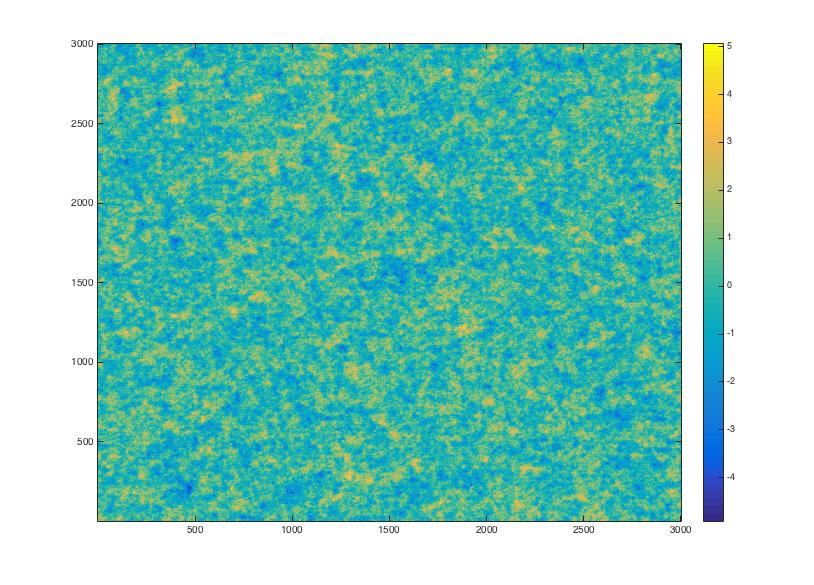
\includegraphics[width = 10cm]{ShadowFieldDeCorr20.jpg}
 \caption{Exponentially correlated shadowing field with $d_{0} = 20m$ (the color of the area refers to the normalized standard deviation which is $S_{i}/\sigma_{s}(i)$)}

 \label{ch4:shadowingfield}
 \end{figure}

 Following the shadowing field generation algorithm, we generate shadowing fields with different values of de-correlation distances. A sample shadowing field is shown in Figure \ref{ch4:shadowingfield} with $20m$ de-correlation distance.

 \par Given a correlated shadowing field, the outage events at different locations are correlated. Without considering other small-scale fading, the channel gain at different locations has a spatial correlation. An outage event occurs when SINR becomes less than $\gamma$, where $\gamma$ is a given SINR threshold. Based on the aforementioned correlated shadow fading model and Random system model, a correlated outage filed can be generated as in Figure \ref{4:outagefie}. On the left, an outage field with independent log-normal shadow fading is shown while the correlated outage field with correlated shadow fading is given on the right. The black color indicates outage areas. The outage area due to independent shadow fading are nonconsecutive dots. In contrast, it contains several connected areas under correlated shadow fading. Therefore, we conclude that correlated shadow fading results in correlated outage areas with regard to a multi-cell system.

 \begin{figure*}
 \centering
 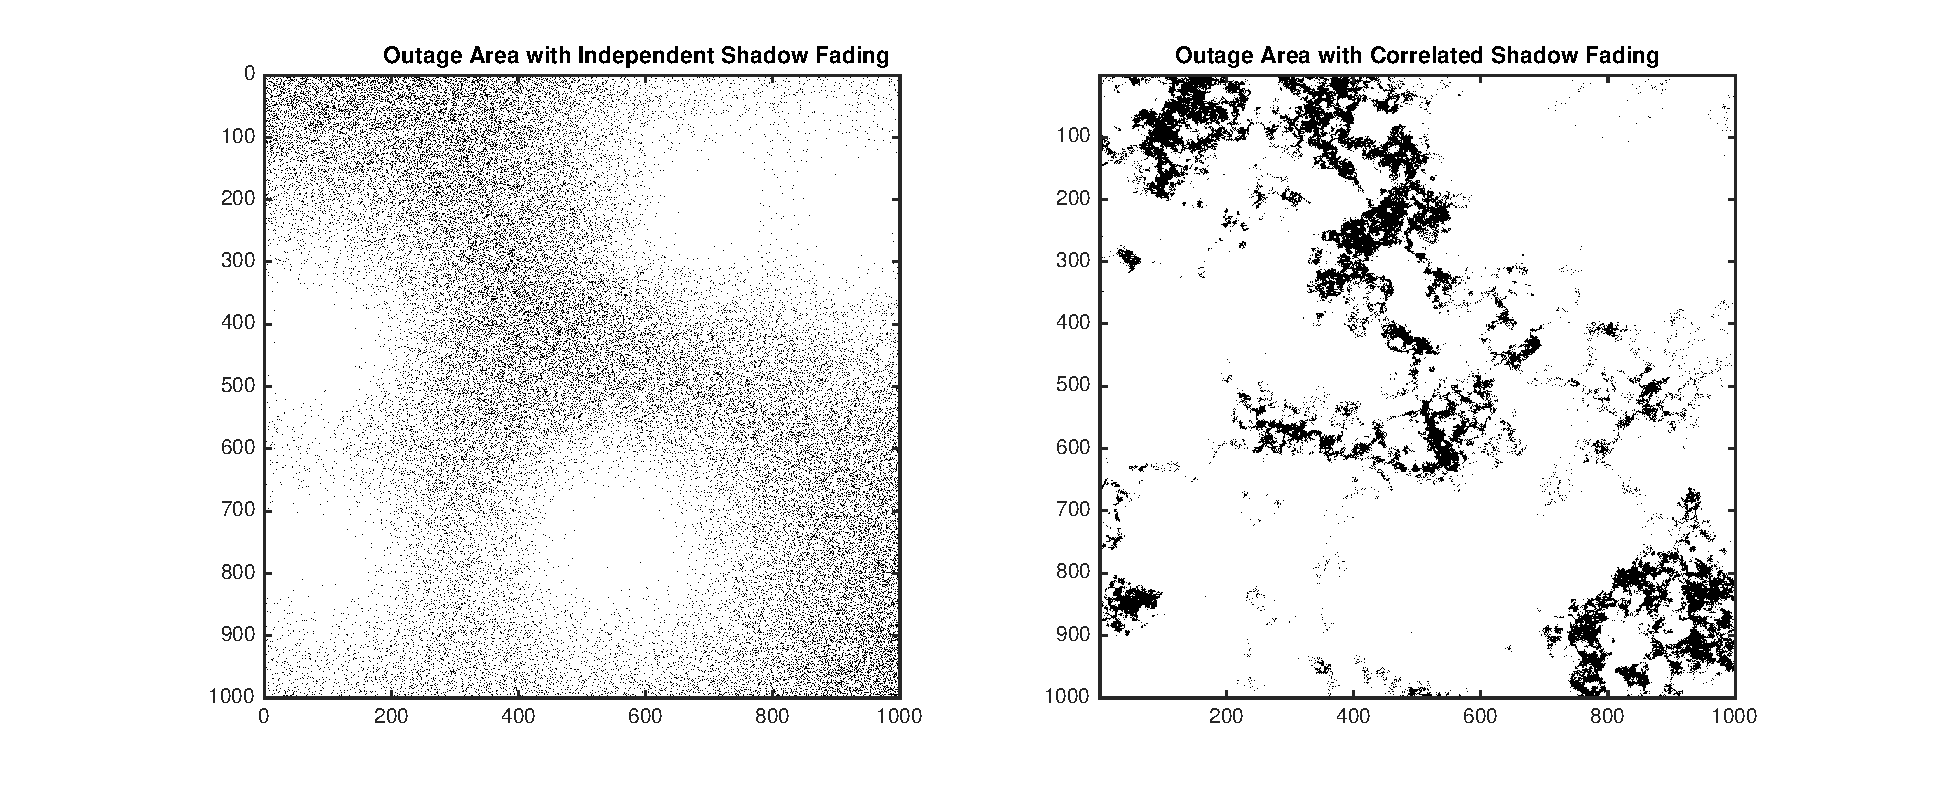
\includegraphics[width=14cm]{outageArea.eps}
 \caption{Correlated outage fields with $\gamma$ (Dark areas are outage areas while white areas are non-outage areas)}
 \label{4:outagefie}
 \end{figure*}


 \section{System Model}
 \label{4:SystemModel}
 In this section, we considered two system models with two different BS deployments: Grid model and Random model.
 \begin{itemize}
 \item Grid model: $\lambda$ BSs are placed on a regular grid deterministically.
 \item Random model: $\lambda$ BSs are placed randomly in a fixed area.
 \end{itemize}
 \begin{figure}
 \centering
 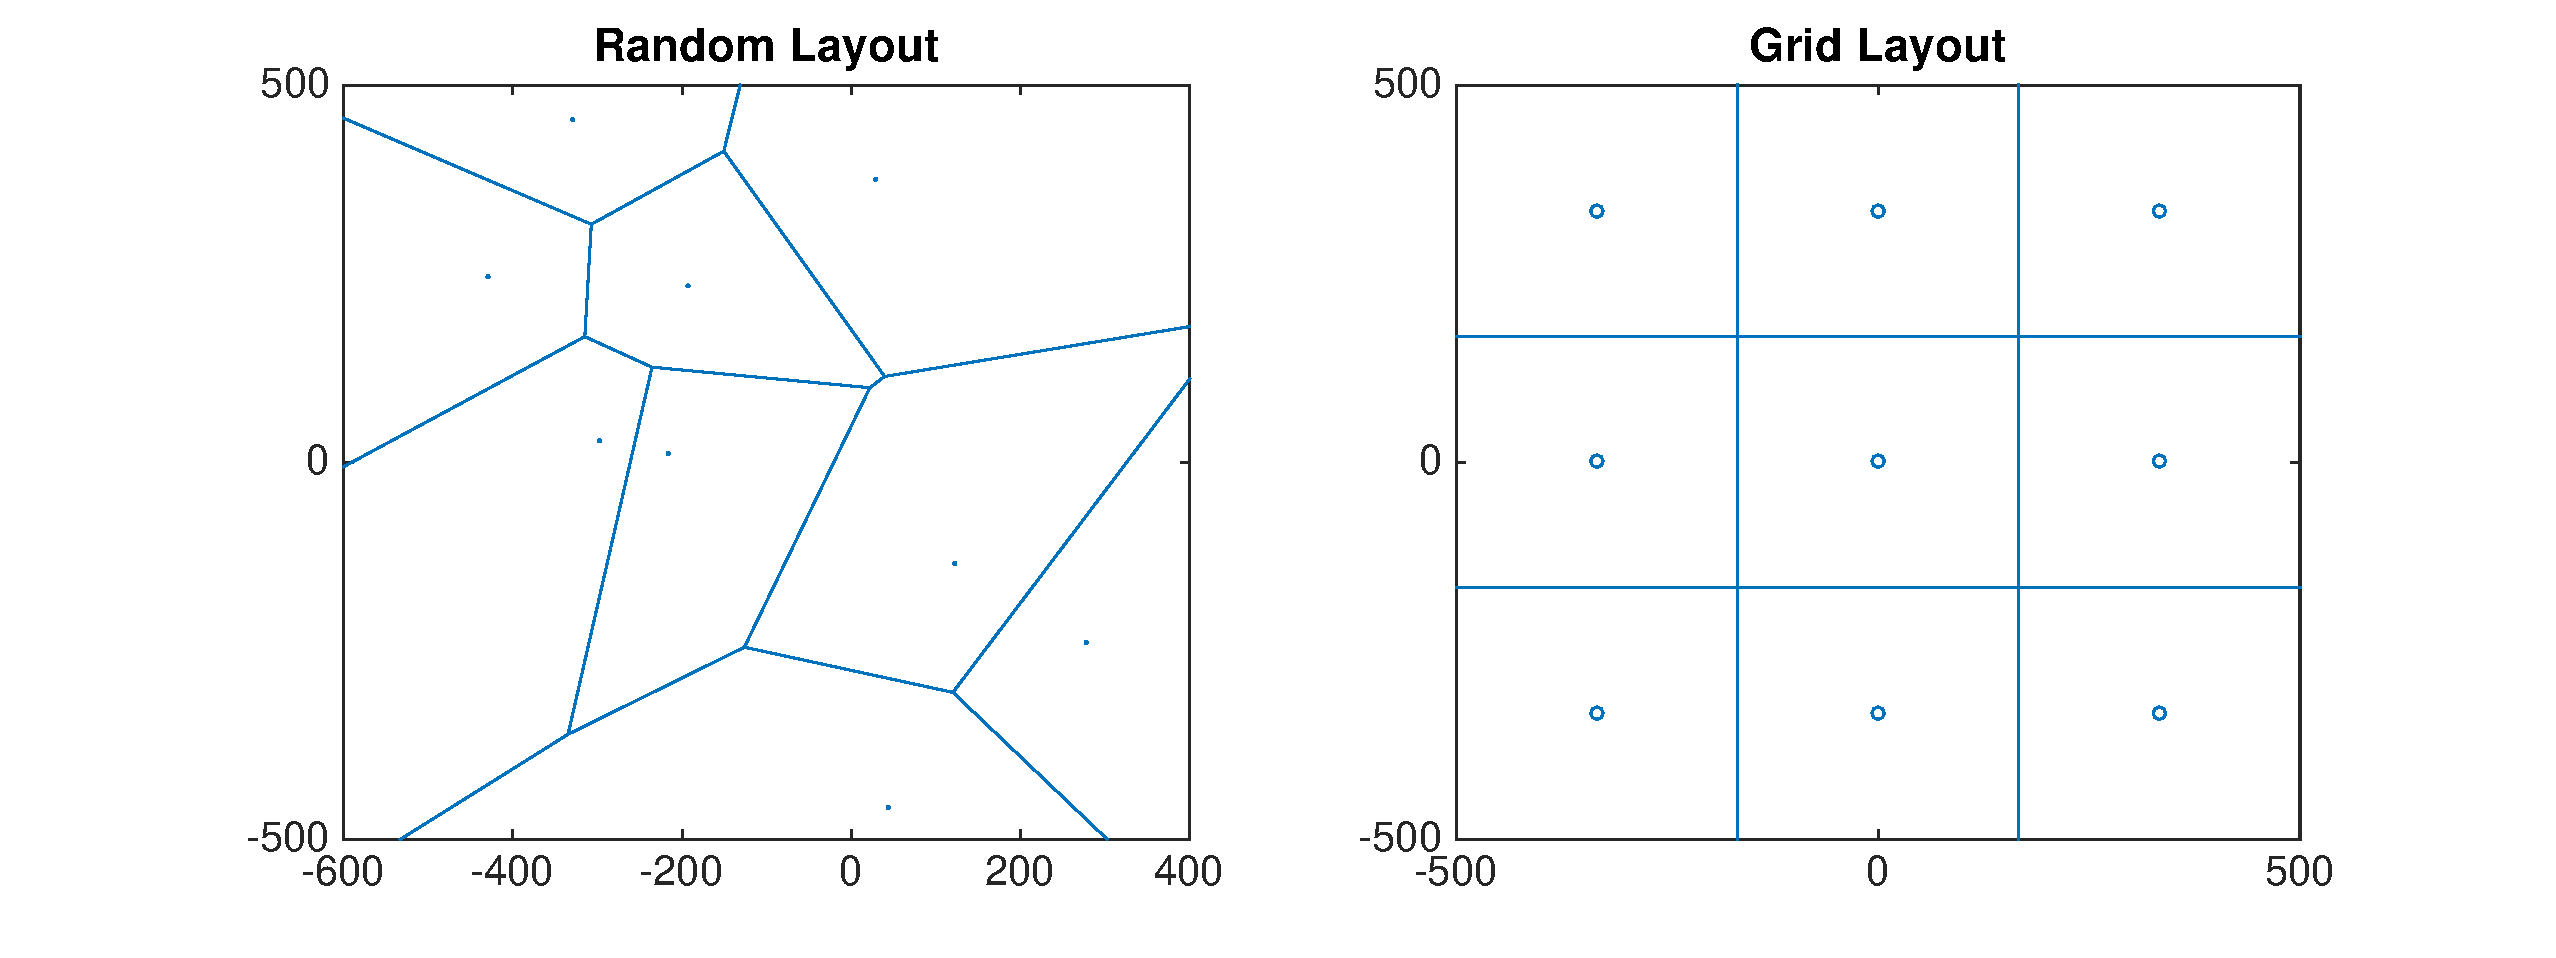
\includegraphics[width=14cm]{systemLayout.eps}
 \caption{Random Layout and Grid Layout with $\lambda = 9$.}
 \label{4:RandomLayout}
 \end{figure}
 % \begin{figure}
 % \centering
 % \includegraphics[width=8cm]{GridLayout.eps}
 % \caption{Grid Base Station Locations}
 % \label{GridLayout}
 % \end{figure}
 Left subfigure of Fig \ref{4:RandomLayout} is an example of a grid model, where cells are in regular square shape with the same size. For the Random model showed in the right subfigure, cells are not guaranteed to be the same shape or same size. Nearest distances between different cells are in a large variation. 


 \section{Outage Probability Analysis}
 \label{4:OutageProb}
 \par Let $\varphi = \{1, 2, \dots, N\}$ denotes the set of all BSs, then the received signal from BS $j$ to the destination user $D$ is given by:
 \begin{equation}
 y_{i\to D} = G_{i\to D}x_{i}+n_{D}.
 \end{equation}
 where $x_{i}$ is the signal transmitted by the source BS and $y_{i\to D}$ is the signal received by the destination user. $n_{D}\sim \mathcal{CN}(0,N_{0})$ is additive white Gaussian noise. $G_{i\to D}$ is the channel gain from source BS to MU including path loss and shadow fading. The end-to-end received $\text{SINR}$ is given in below:
 \begin{equation}
 \text{SINR} \triangleq \frac{P_{i}*G_{i\to D}^{2}}{N_{0}+\sum_{j\in \varphi/i}P_{j}*G_{j\to D}^2},
 \end{equation}
 where $P_{i}$ is the transmitted power of BS $i$. The MU successfully receives the signal if no outage event occurs, i.e., $\log_{2}(1+\text{SINR})\ge R$, where $R$ is the required data rate. From the definition of SINR, no outage event occurs as long as $\text{SINR} > \gamma$, where $\gamma = 2^{R}-1$.

 \par For a particular MU, outage event occurs when its received SINR is less than a threshold to decode the received signal. In our scenario, the probability that the receiver cannot decode signals received from its serving BS is defined as:
 \begin{equation}
 P(out_{i}) = P[\text{SINR}_{i\to D} < \gamma],
 \end{equation}
 We investigate two connection strategies: 
 \begin{itemize}
 \item Nearest BS: MU choose to connect to the nearest BS.
 \item Strongest BS: MU choose to connect to the BS with highest SINR.
 \end{itemize}
 \par In Nearest BS mode, we assume that the MU is served by the nearest BS, then the outage probability will be 
 \begin{equation}
 P_{out} = P_{out_{i}},
 \end{equation} 
 where $i$ is the index of the nearest Base Station. 
 \par In Strongest BS mode, under the assumption that an MS always connecting to the BS which provides the highest SINR, the outage event occurs if no BS can provide high enough SINR to the receiver. Based on this assumption we have:
 \begin{equation}
 P_{out} = \max_{i = 1,\cdots,N} P[\text{SINR}_{i\to D}<\gamma].
 \end{equation}
 The probability density function (pdf) of shadow fading $S$ given $L$ correlated fading branches is
 \begin{equation}
 \begin{split}
 f_{\mathbf{S}}(\mathbf{s}) = &\frac{\lambda^{L}}{\sqrt{2\pi}|\mathbf{K}_{L\times L}|^{1/2}\prod_{i=1}^{L}s_{i}}\\
 &\cdot\exp(-\frac{1}{2}(10\log_{10}\mathbf{s}-\boldsymbol{\mu})^{T}\mathbf{K}_{L\times L}^{-1}(10\log_{10}\mathbf{s}-\boldsymbol{\mu})),
 \end{split}
 \end{equation}
 where $\lambda = 10/\ln10$ and $\boldsymbol{\mu}$ is the average shadow fading which is normally $0$. $\mathbf{K}_{L\times L}$ is the correlation matrix which is defined in \eqref{correlationmatrix}. Let $\theta_{i} = \frac{10\log_{10}s_{i}-\mu_{i}}{\sqrt{2}\sigma_{i}}$, and doing a change of variables gives us the pdf of $\mathbf{\Theta}$ as follows:
 \begin{equation}
 f_{\mathbf{\Theta}}(\boldsymbol{\theta}) = \frac{1}{\pi^(L/2)|\mathbf{\Sigma}|^{1/2}}\exp(-\mathbf{\Theta}^{T}\mathbf{\Sigma}^{-1}\mathbf{\Theta}),
 \end{equation}
 where $\mathbf{\Sigma}$ is the correlation coefficient matrix which is
 \begin{equation}
 \left[\begin{array}{cccc}
 1 & h_{1,2} & \cdots & h_{1,L}\\
 \vdots & \ddots & \ddots & \vdots\\
 h_{L,1} & h_{L,2} & \cdots & 1\\
 \end{array}\right].
 \end{equation}
 Since $\text{SINR}_{i\to D}=PL_{i\to D}+S_{i}-N_{0}-\sum_{j\in\varphi/i}(PL_{j\to D} + S_{j})$ in dB, $\text{SINR}_{i\to D}<\gamma$ means
 \begin{equation}
 S_{i} - \sum_{j\in\varphi/i}S_{j}<\gamma -PL_{i\to D} + \sum_{j\in\varphi/i}PL_{j\to D} + N_{0},
 \end{equation}
 where $\varphi$ denotes the set of all BSs.
 Then the outage probability can be written as:
 \begin{equation}
 \label{4:outprob}
 P_{out} = \underbrace{\int_{-\infty}^{+\infty}\cdots\int_{-\infty}^{+\infty}}_{i =1,\cdots,N} g(PL_{i}S_{i} - \gamma\sum_{j\in\varphi/i}PL_{j}S_{j})f(\mathbf{s})d\mathbf{s}.
 \end{equation}
 where $\mathbf{s}$ is the correlated shadow fading experienced by all BSs, $g(PL_{i}S_{i} - \gamma\sum_{j\in\varphi/i}PL_{j}S_{j})$ is a step function defined in (\ref{4:stepfunction}). 
  \begin{figure}[!t]
 % ensure that we have normalsize text
 \normalsize
 % Store the current equation number.
 % \setcounter{MYtempeqncnt}{\value{equation}}
 % % Set the equation number to one less than the one
 % % desired for the first equation here.
 % % The value here will have to changed if equations
 % % are added or removed prior to the place these
 % % equations are referenced in the main text.

 \begin{equation}
 \label{4:stepfunction}
 g(PL_{i}S_{i} - \gamma\sum_{j\in\varphi/i}PL_{j}S_{j}) = \{\begin{array}{cc}
                1, &  \text{  when }PL_{i}S_{i} - \gamma\sum_{j\in\varphi/i}PL_{j}S_{j} <\frac{\gamma N_{0}}{P}\\
                0, & \text{  when }PL_{i}S_{i} - \gamma\sum_{j\in\varphi/i}PL_{j}S_{j} >\frac{\gamma N_{0}}{P}
              \end{array}.
 \end{equation}
 % Restore the current equation number.
 % \setcounter{equation}{\value{MYtempeqncnt}}
 % IEEE uses as a separator
 \hrulefill
 % The spacer can be tweaked to stop underfull vboxes.
 \vspace*{4pt}
 \end{figure}

 \section{Simulation Results}
 \label{4:SimuProb}
 \par In this section, we will present simulation setup and results. Firstly, we run simulations to compare the outage probability of the two different network topologies: Grid model and Random model. Secondly, SINR distribution and outage probability of Random model given different BS densities are investigated. Two scenarios are considered: MU connecting to the nearest BS and MU connecting to the BS providing highest SINR. At the end, the outage duration distribution are simulated and discussed given different BS densities. The simulation parameters are presented in Table \ref{SystemConfig2}. 
 \begin{table}
 \centering
 \caption{\label{SystemConfig2}Simulation Configuration Parameters}

 \begin{tabular}{|c|c|}

 \hline
 Study Area & $1000m\times 1000m$\\
 \hline
 BS Densities & $3, 10, 50, 100, 200, 300, 500$\\
 \hline
 Path Loss Exponent & $4$\\
 \hline
 BS Transmission Power & $P: 40dbm$\\
 \hline
 SNR Requirement & $-5dB$\\
 \hline
 De-Correlation Distance & $20m, 200m$\\
 \hline
 \end{tabular}

 \end{table}

 \par Figure \ref{4:cdf1} shows the Cumulative Distribution Function (CDF) of SINR when MU is connecting to the nearest BS. The de-correlation distance of the correlated shadow fading is $20m$. The figure suggests that Grid model outperforms the Random model, which is consistent with findings in \cite{andrews2011tractable}. Figure \ref{4:outage1} shows the outage probability with SINR threshold being $-5dB$. The outage probability of Grid Layout (blue) is lower than that of the Random Layout (yellow). In next section, we will focus on the Random model which is more realistic than Grid model.
 \begin{figure}
 \centering
 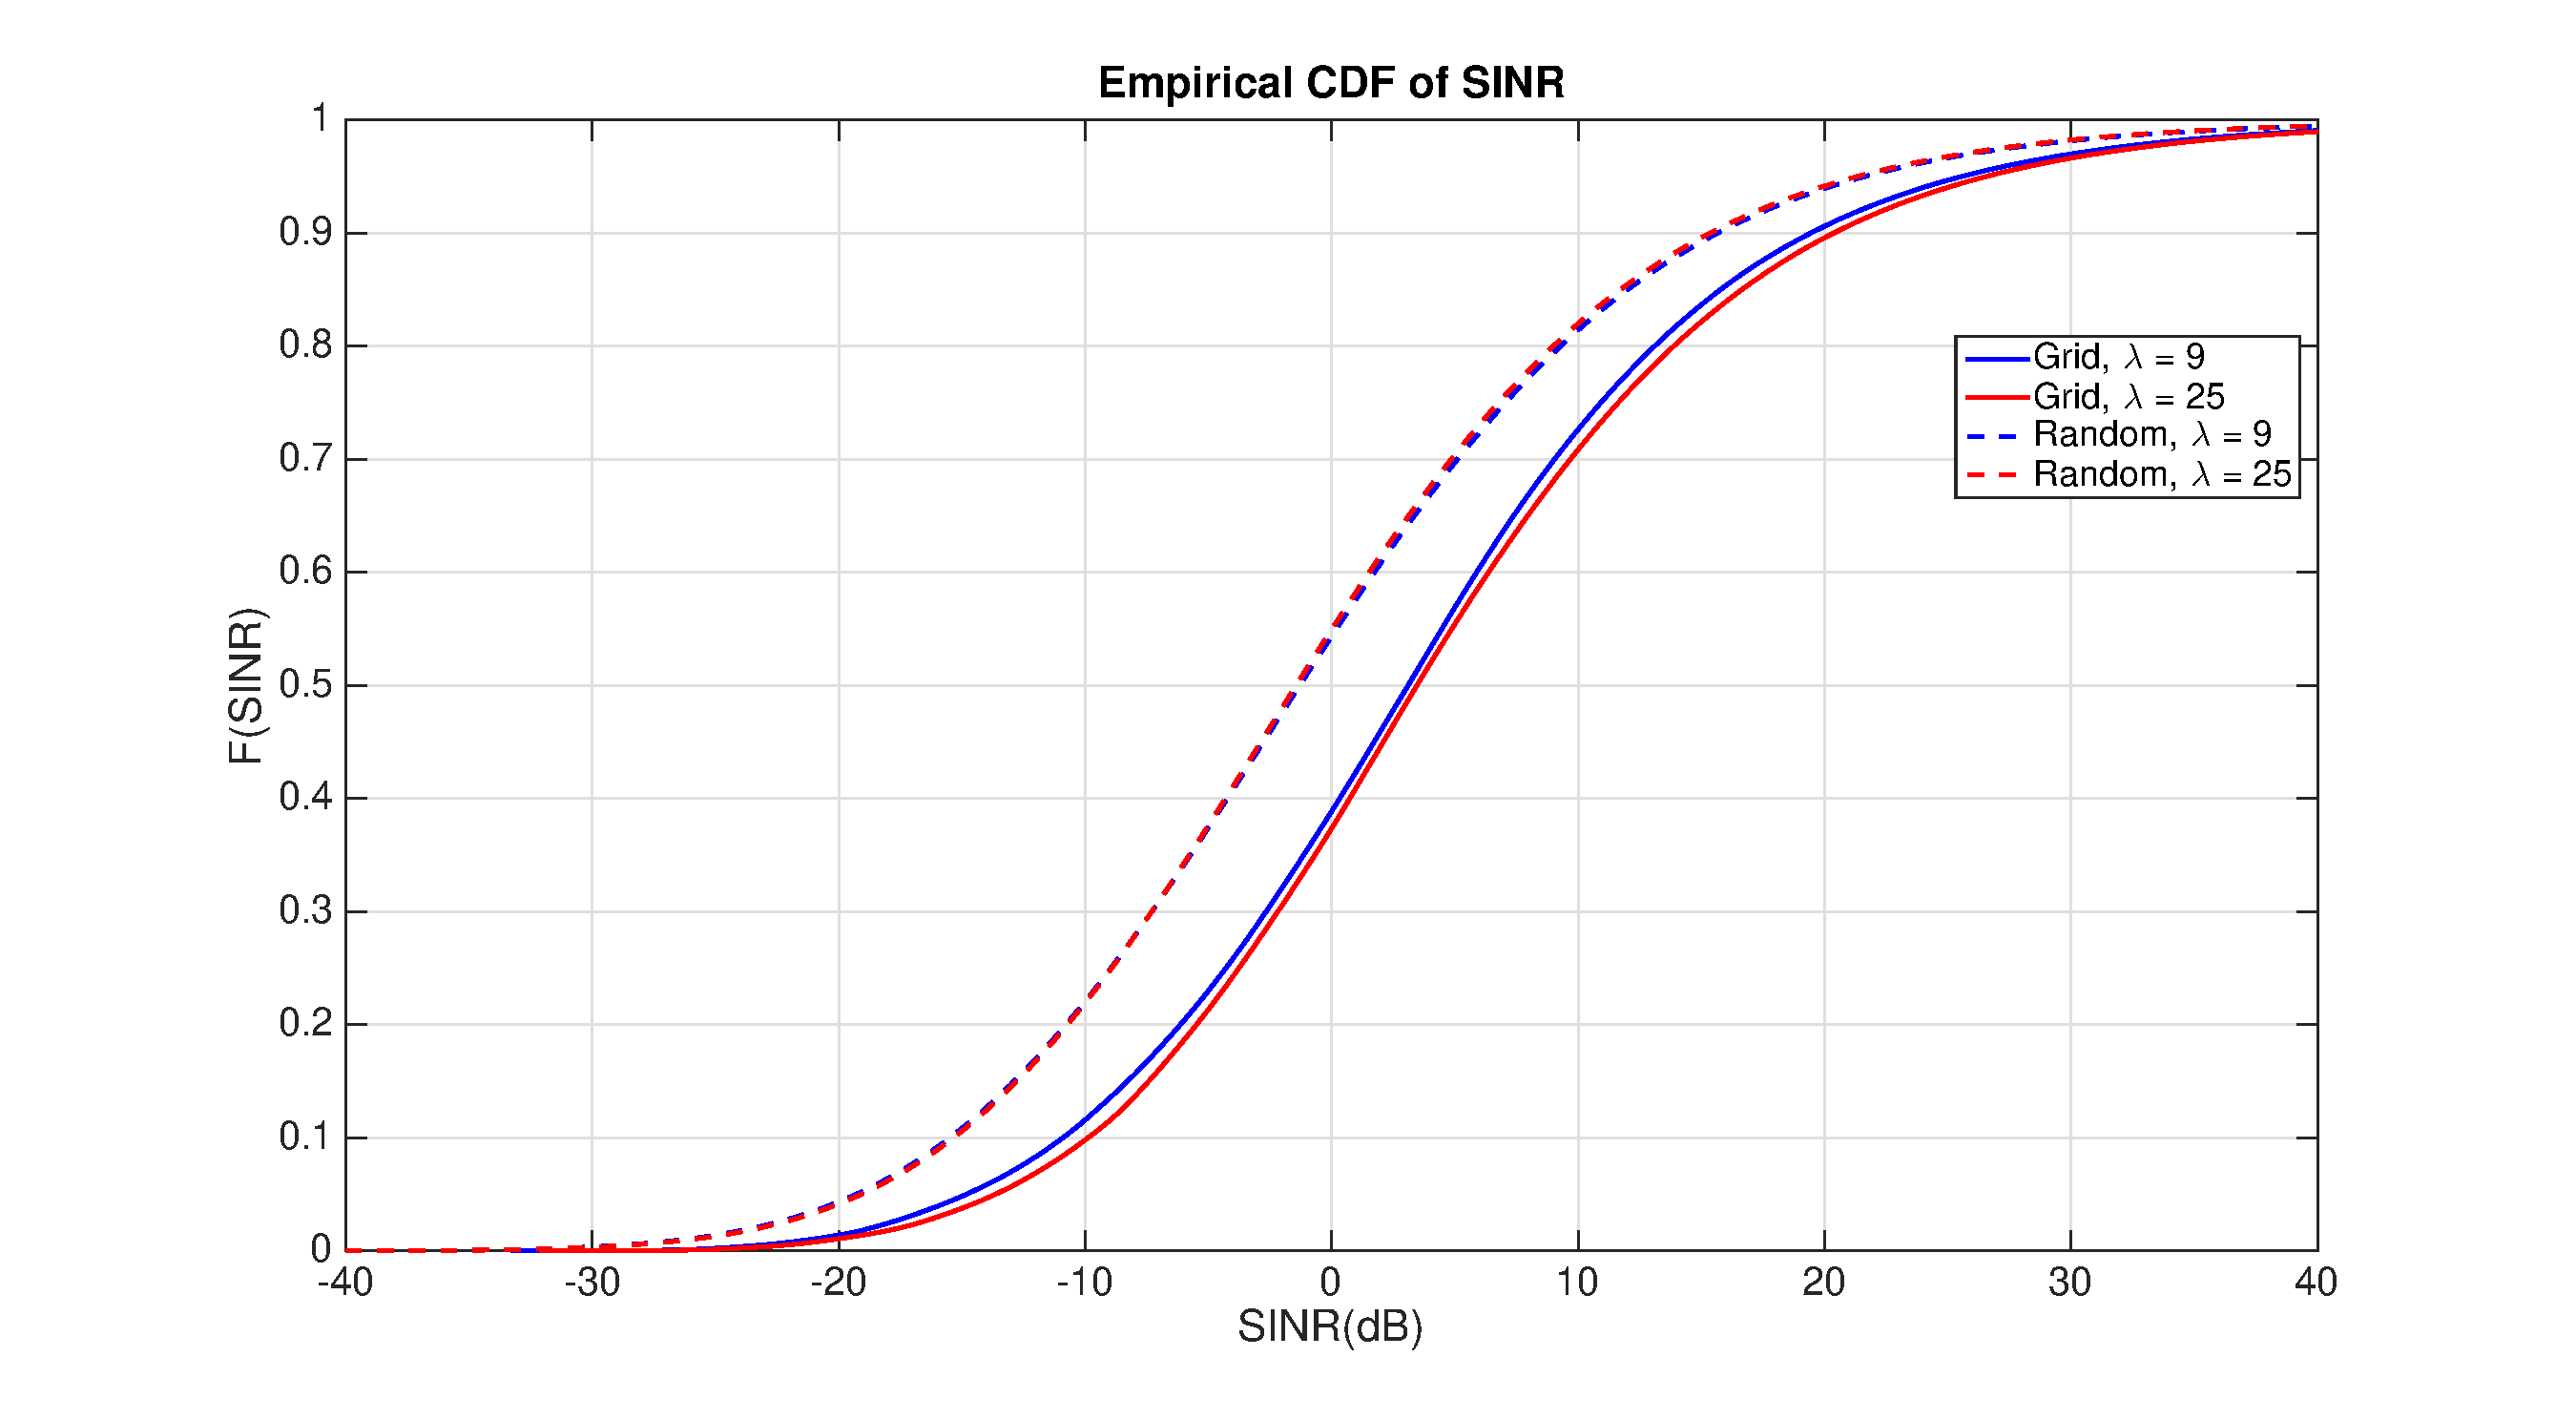
\includegraphics[width=10cm]{GridVSRandom.eps}
 \caption{CDF of SINR given Grid Layout and Random Layout (De-Correlation Distance: $20m$)}
 \label{4:cdf1}
 \end{figure}
 \begin{figure}
 \centering
 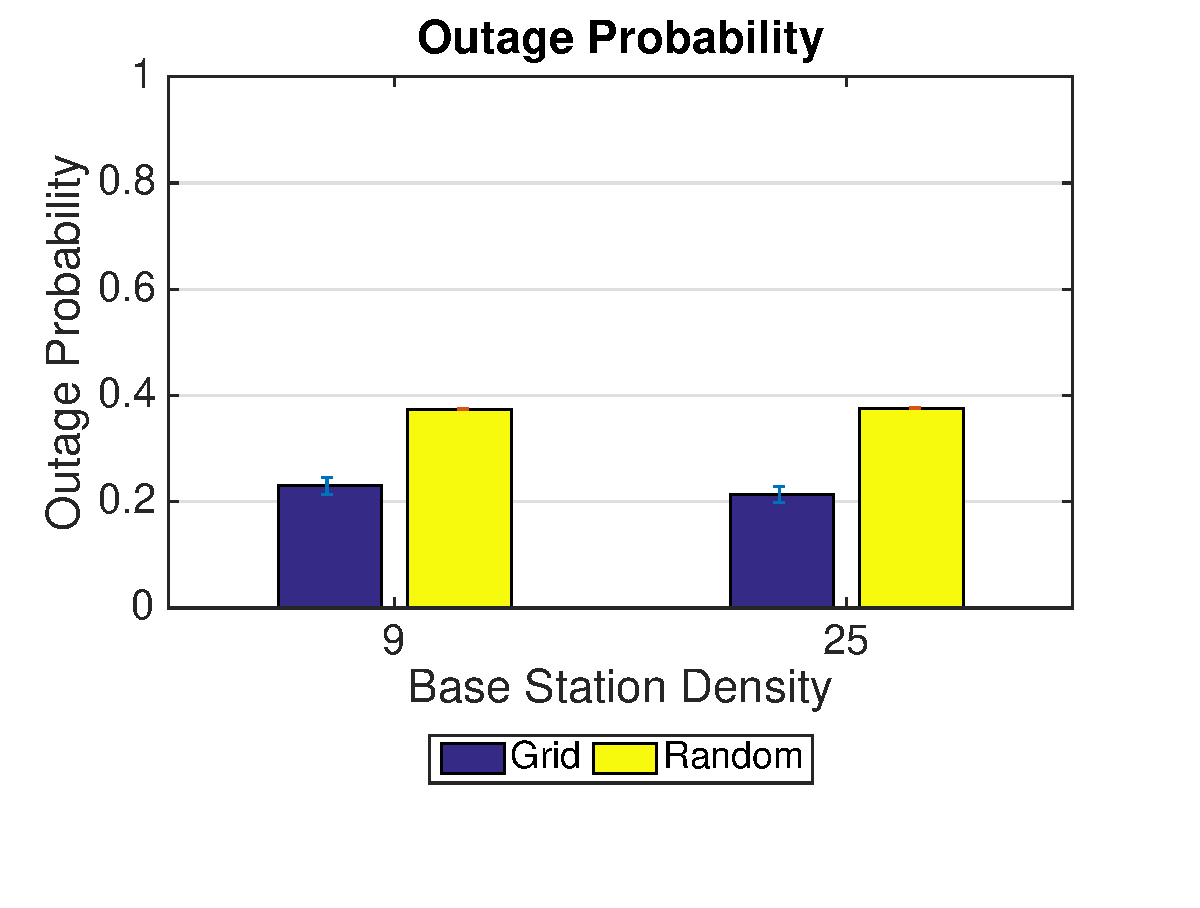
\includegraphics[width=10cm]{OutageProbGridVSRandom.eps}
 \caption{Outage Probability given Grid Layout and Random Layout (De-Correlation Distance: $20m$)}
 \label{4:outage1}
 \end{figure}


 \begin{figure}
 \centering
 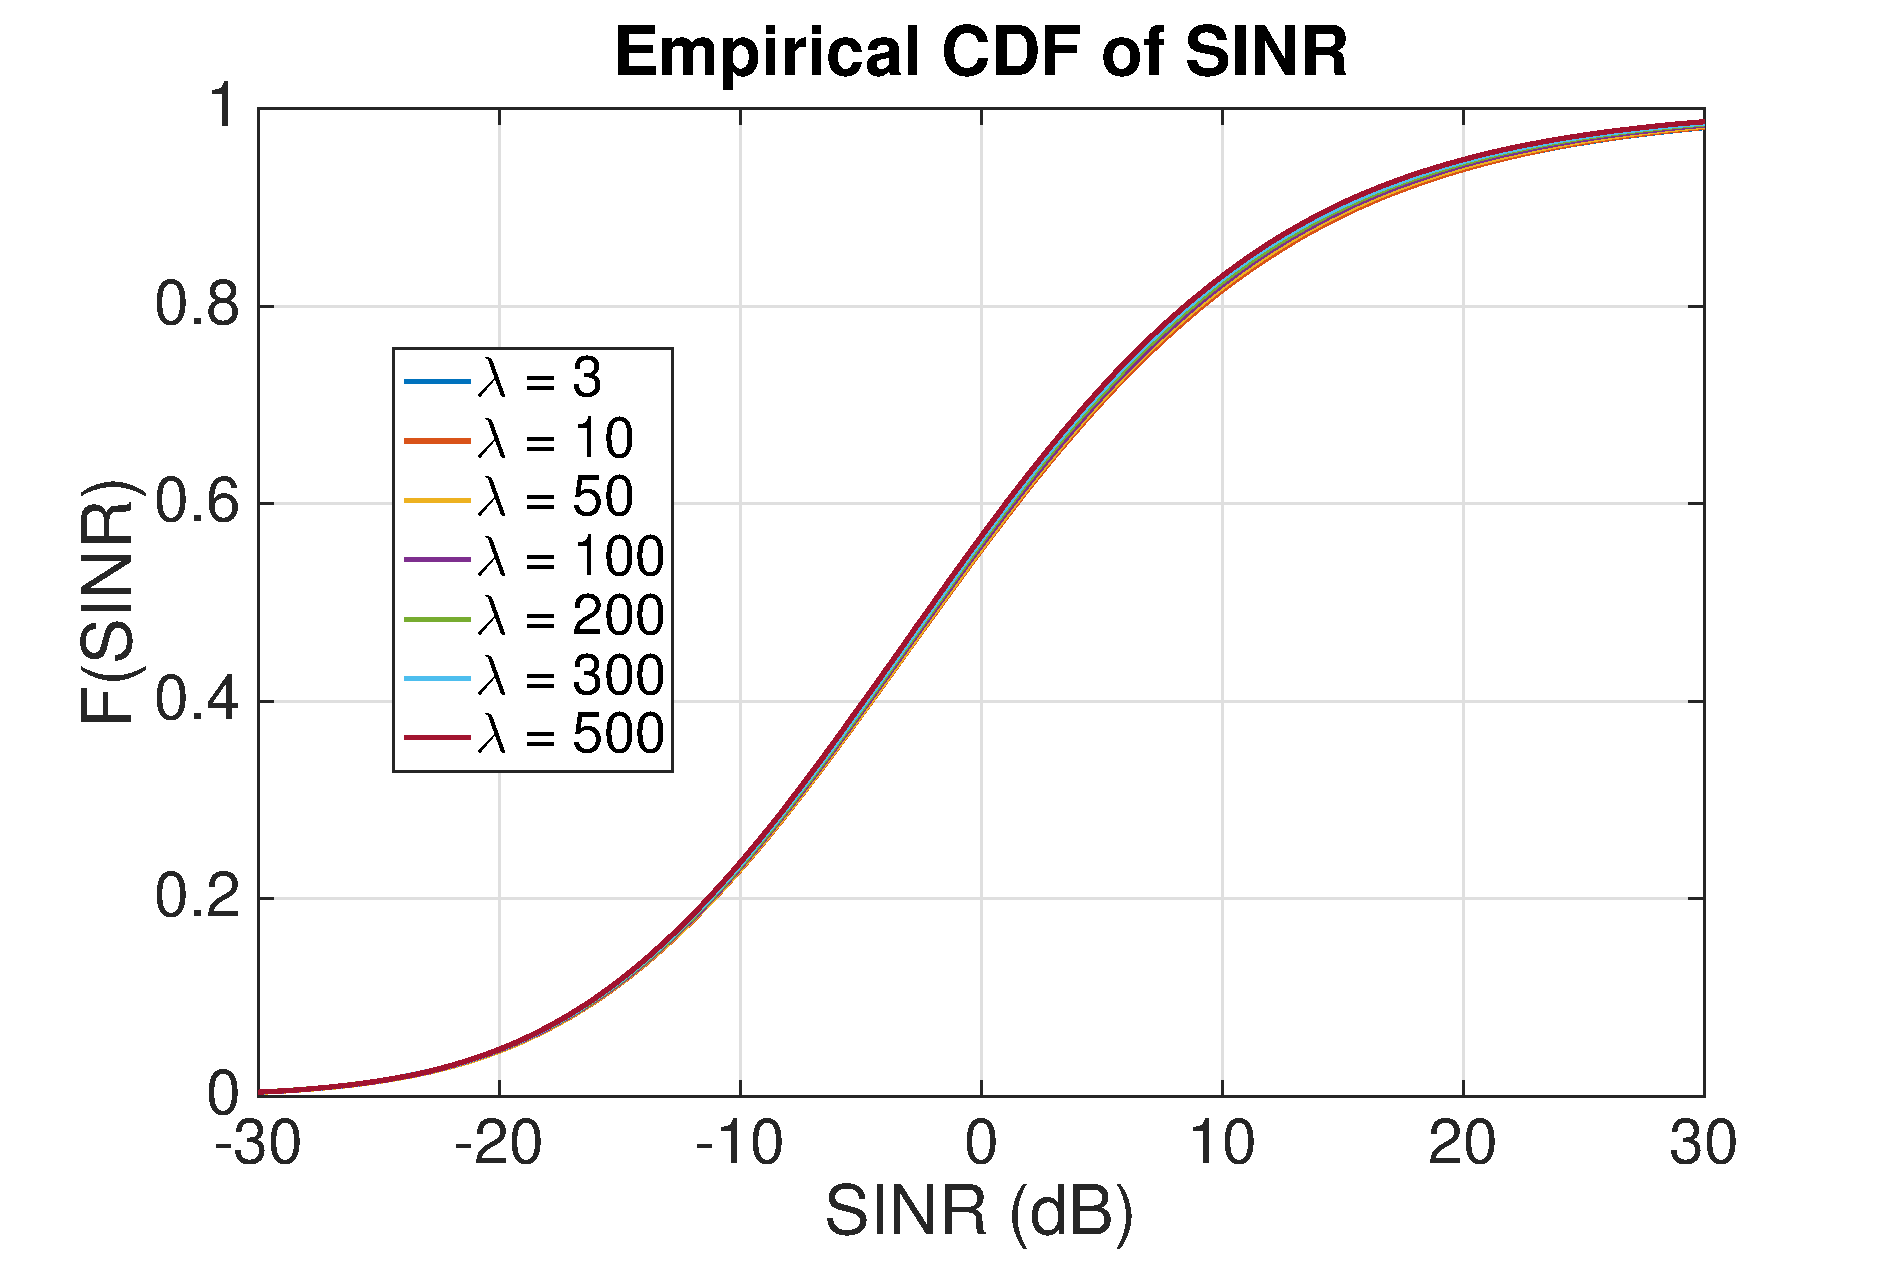
\includegraphics[width=10cm]{NBMax1000OutageProbCDFiid.eps}
 \caption{CDF of SINR of MU when connecting to the nearest BS. i.i.d. Shadow Fading}
 \label{4:Mode1}
 \end{figure}
 \begin{figure}
 \centering
 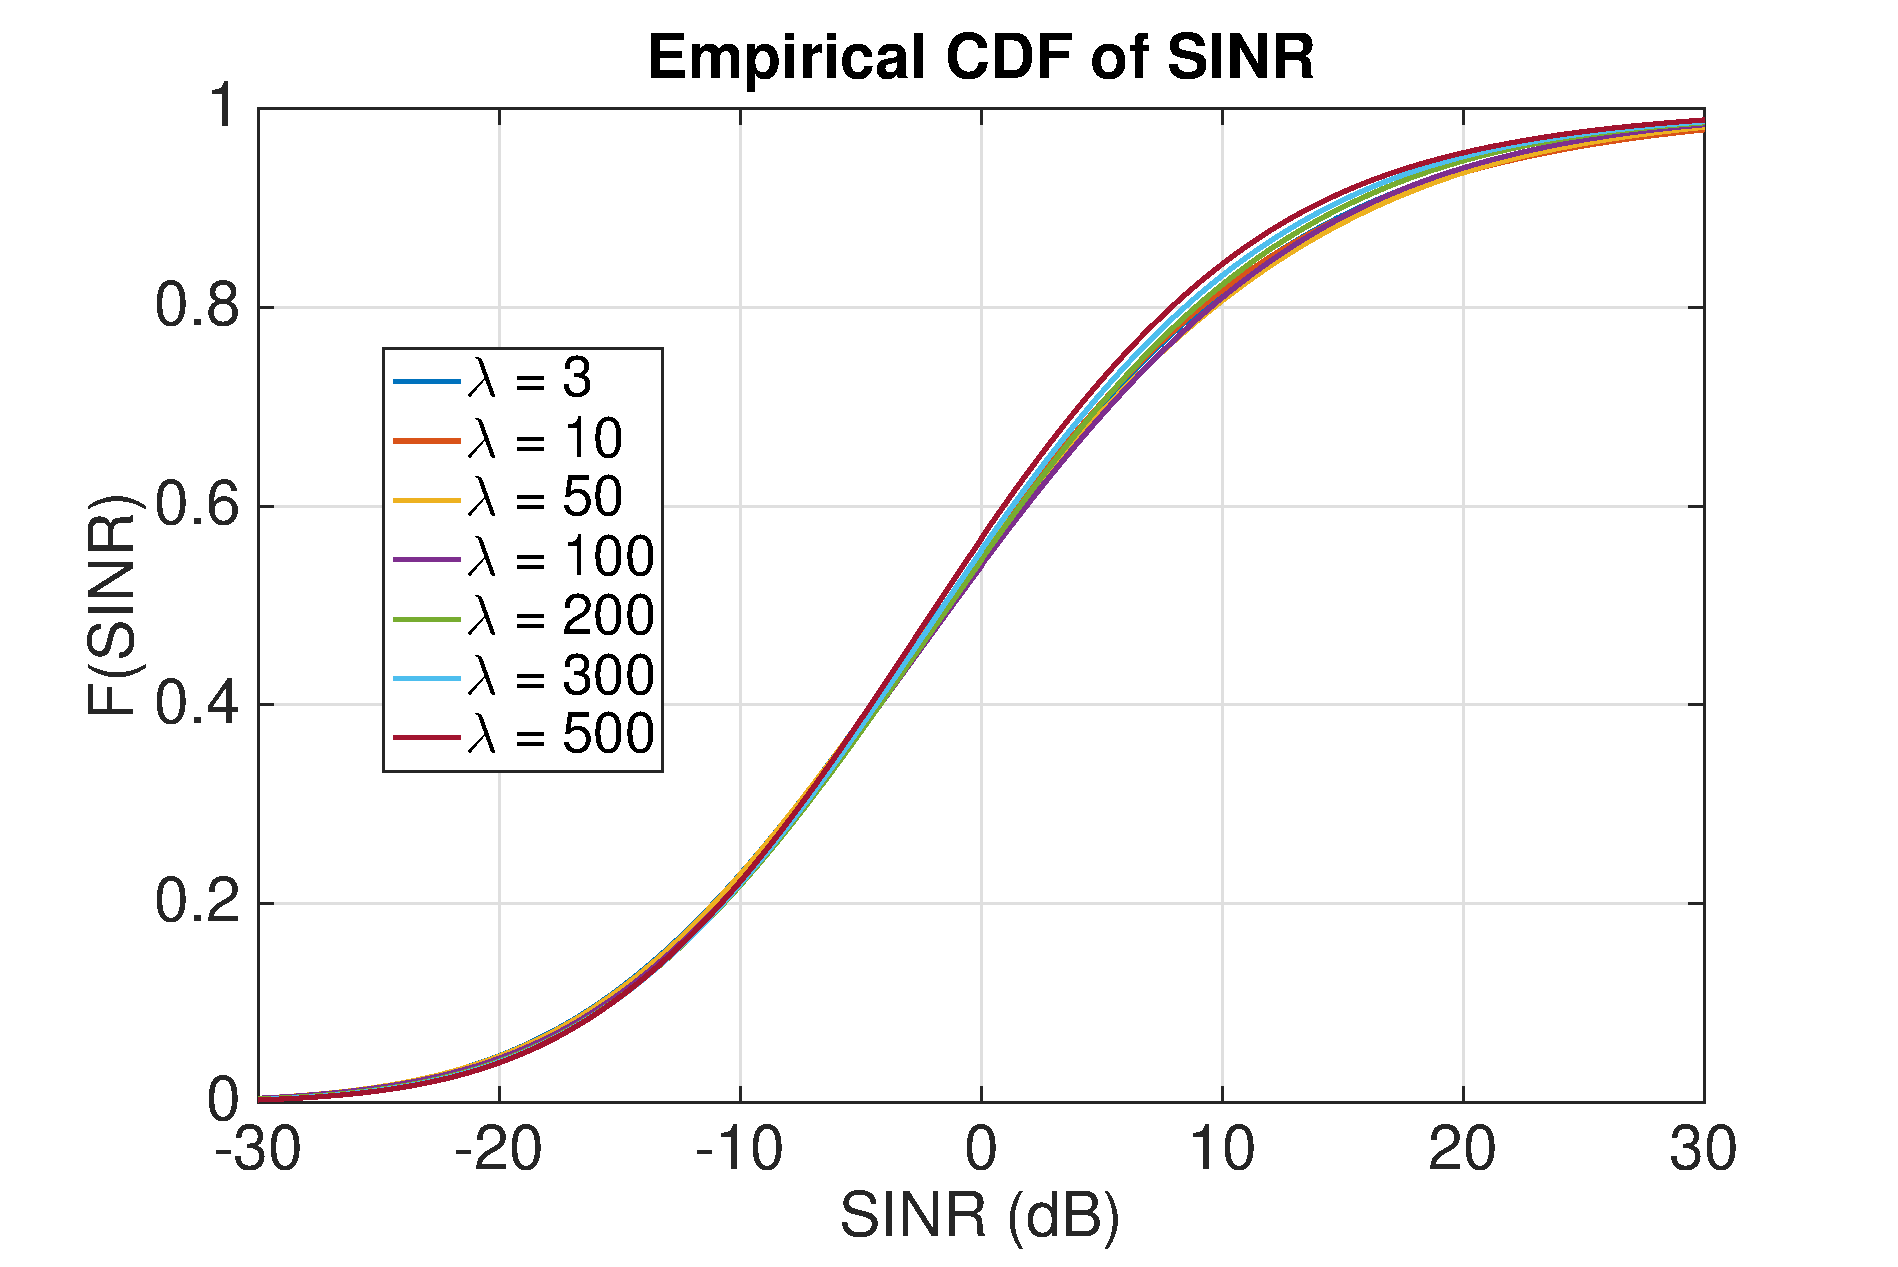
\includegraphics[width=10cm]{NBMax1000OutageProbCDFDeCorr20.eps}
 \caption{CDF of SINR of MU when connecting to the nearest BS. De-Correlation Distance: 20m}
 \label{4:Mode2}
 \end{figure}
 \begin{figure}
 \centering
 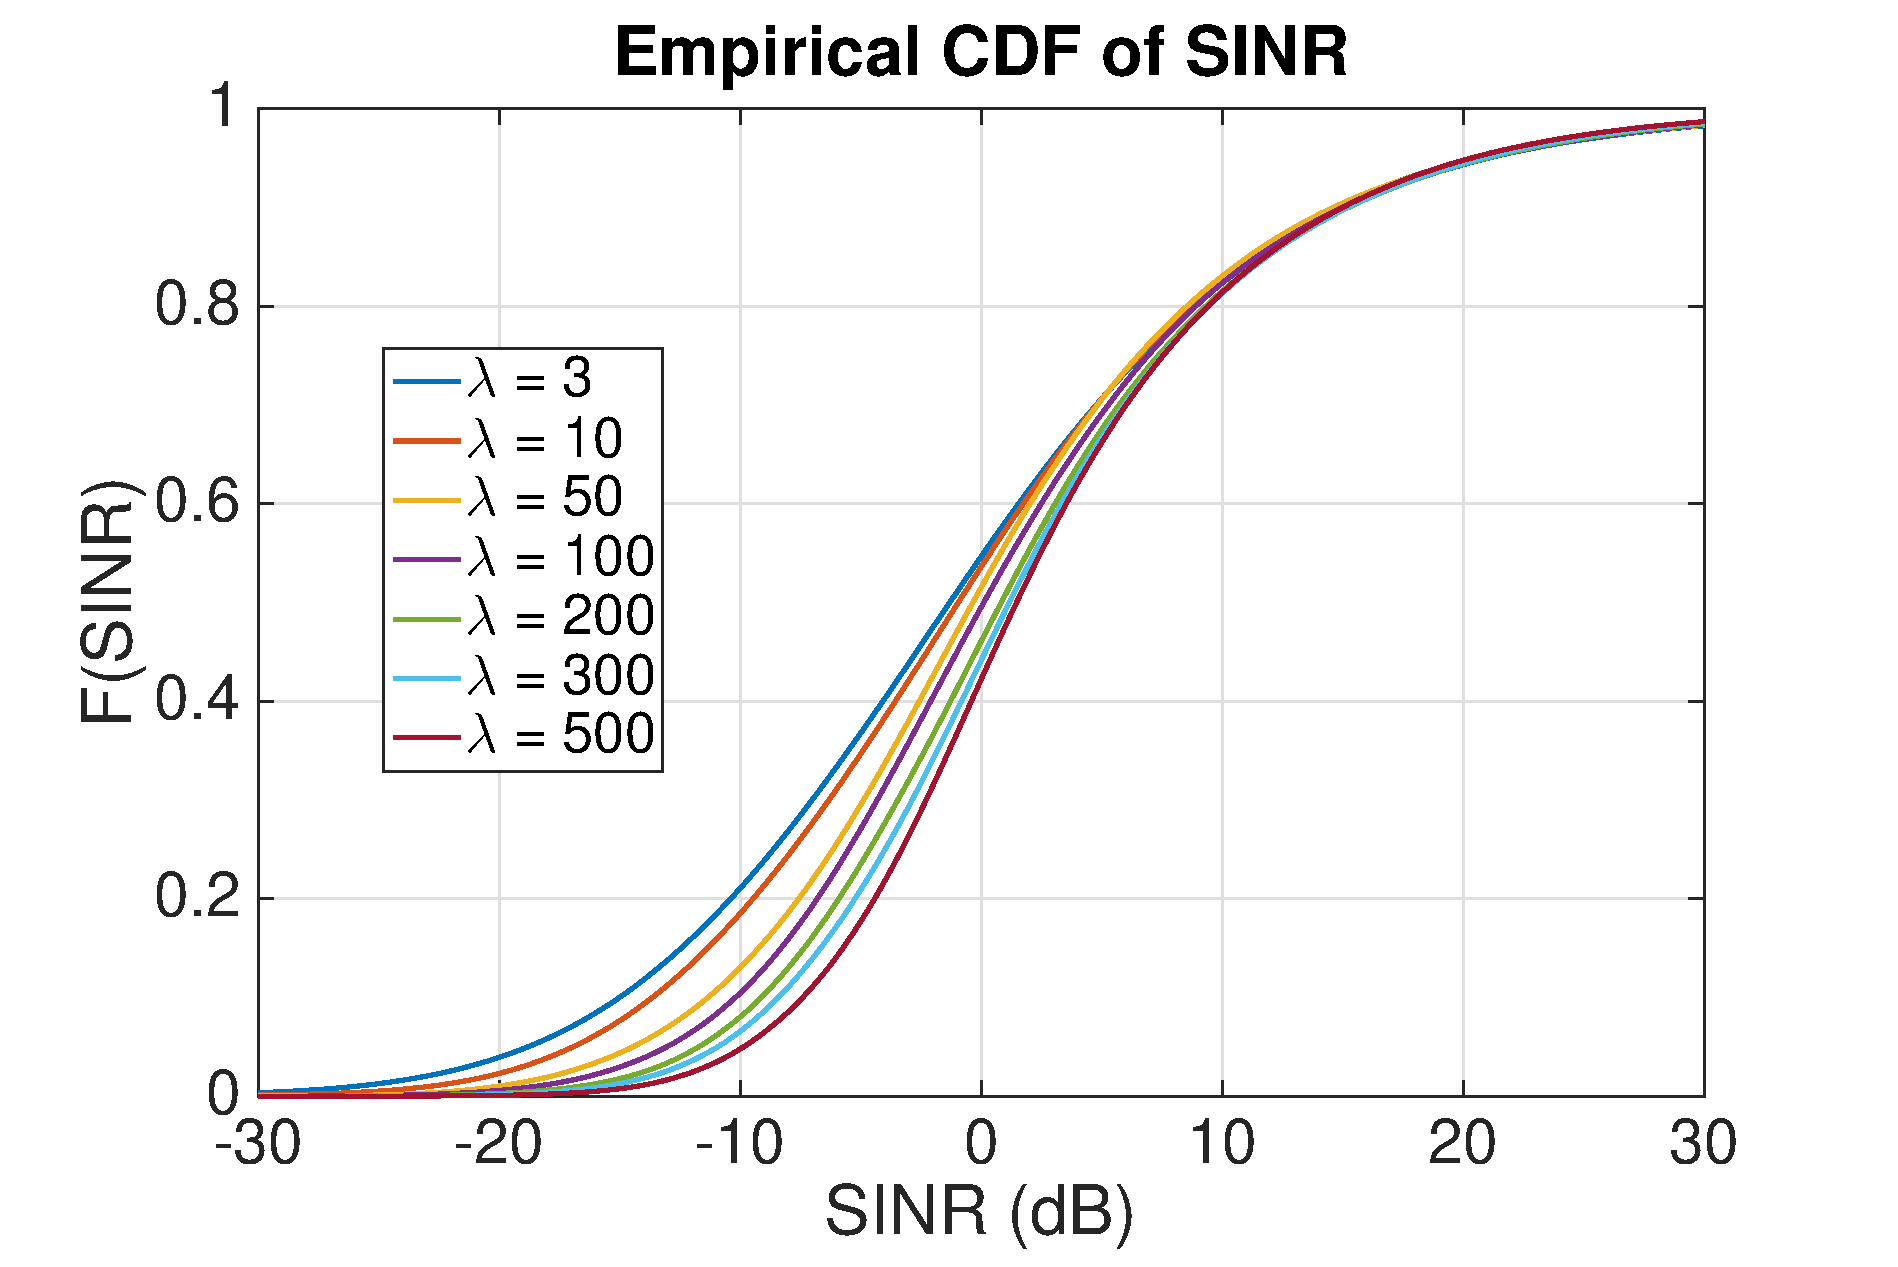
\includegraphics[width=10cm]{NBMax1000OutageProbCDFDeCorr200.eps}
 \caption{CDF of SINR of MU when connecting to the nearest BS. De-Correlation Distance: 200m}
 \label{4:Mode3}
 \end{figure}


 \begin{figure}
 \centering
 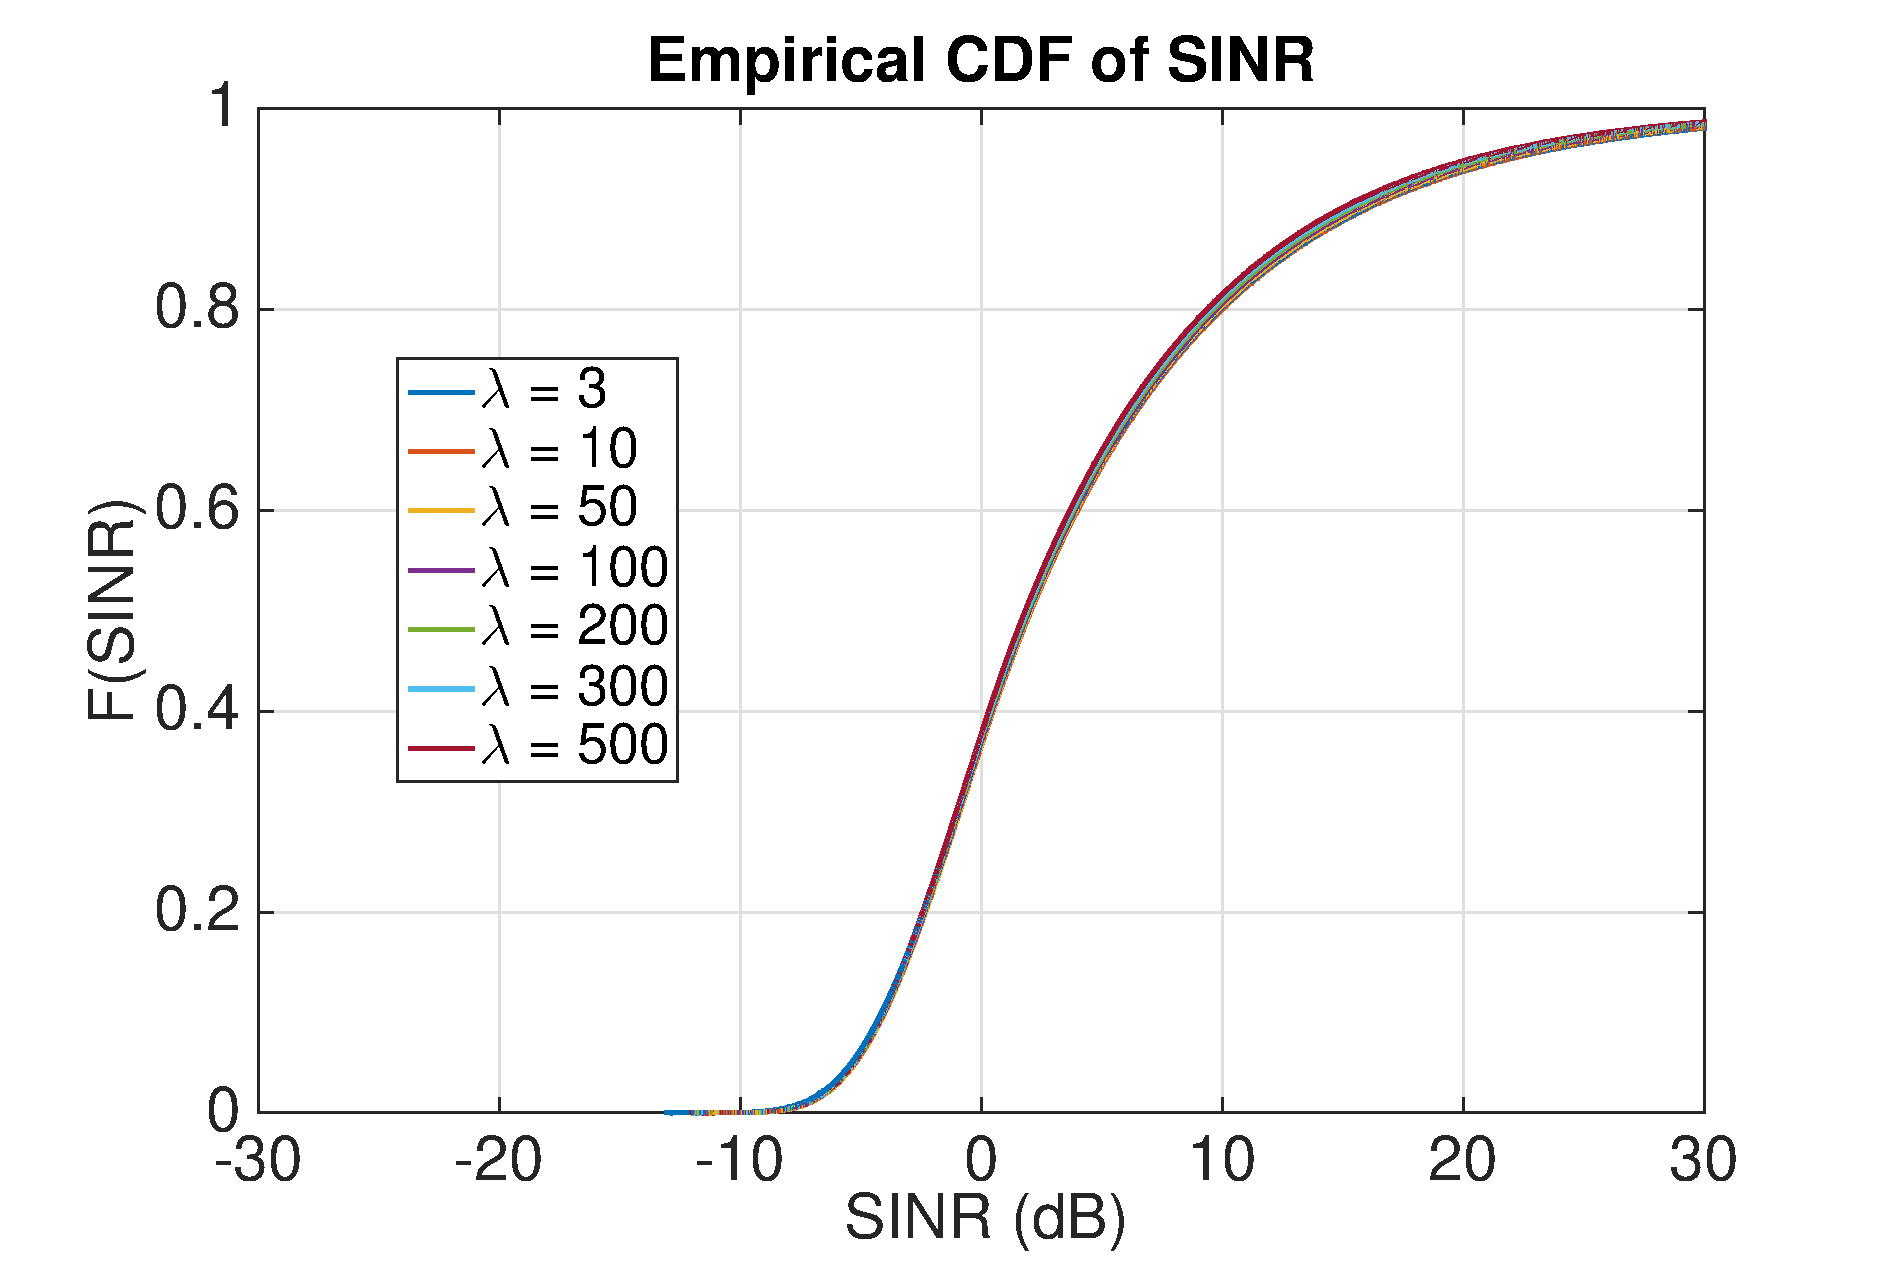
\includegraphics[width=10cm]{MaxMax1000OutageProbCDFiid.eps}
 \caption{CDF of SINR of MU when connecting to the strongest BS. i.i.d. Shadow Fading}
 \label{4:Mode12}
 \end{figure}
 \begin{figure}
 \centering
 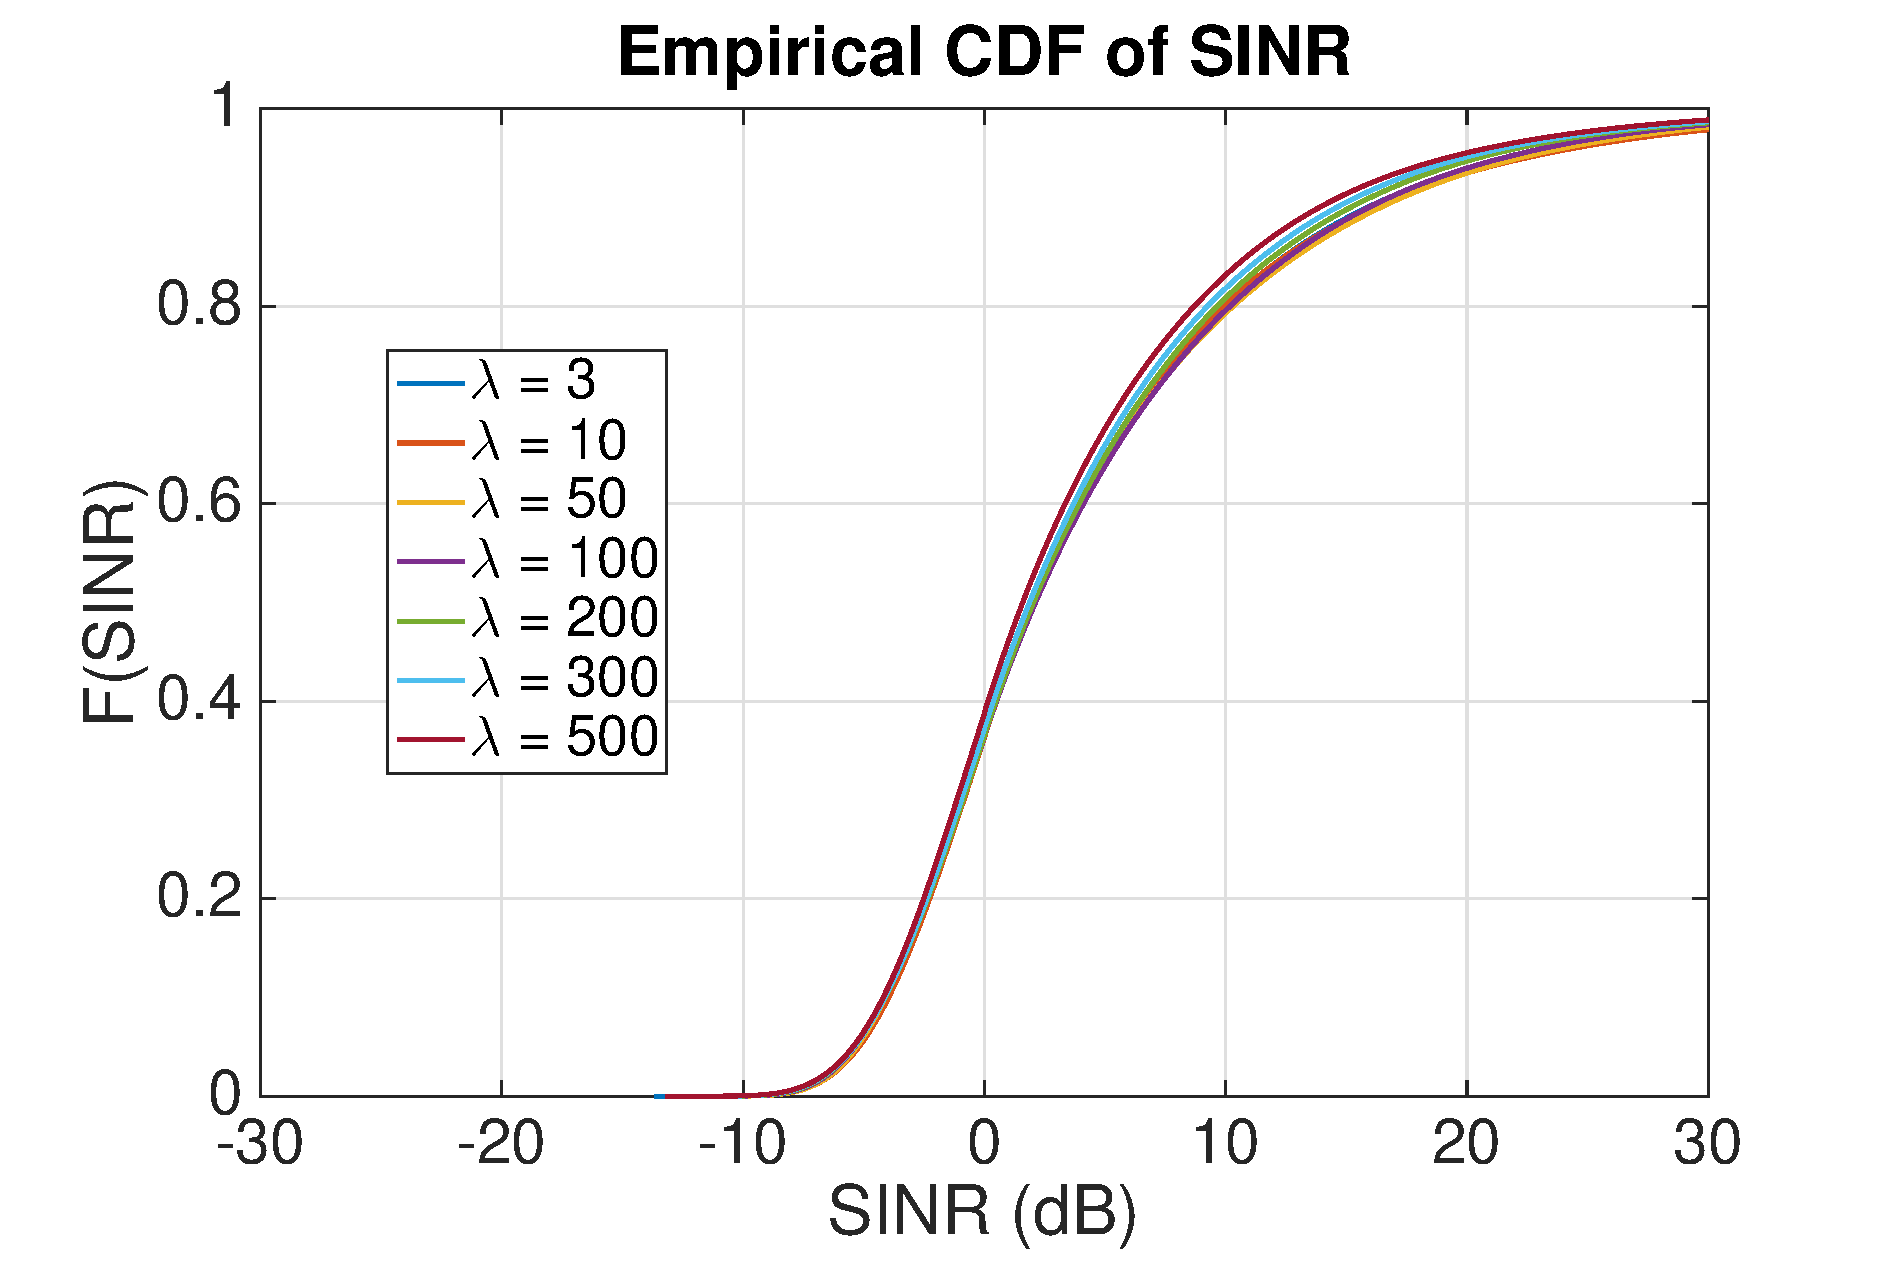
\includegraphics[width=10cm]{MaxMax1000OutageProbCDFDeCorr20.eps}
 \caption{CDF of SINR of MU when connecting to the strongest BS. De-Correlation Distance: 20m}
 \label{4:Mode22}
 \end{figure}
 \begin{figure}
 \centering
 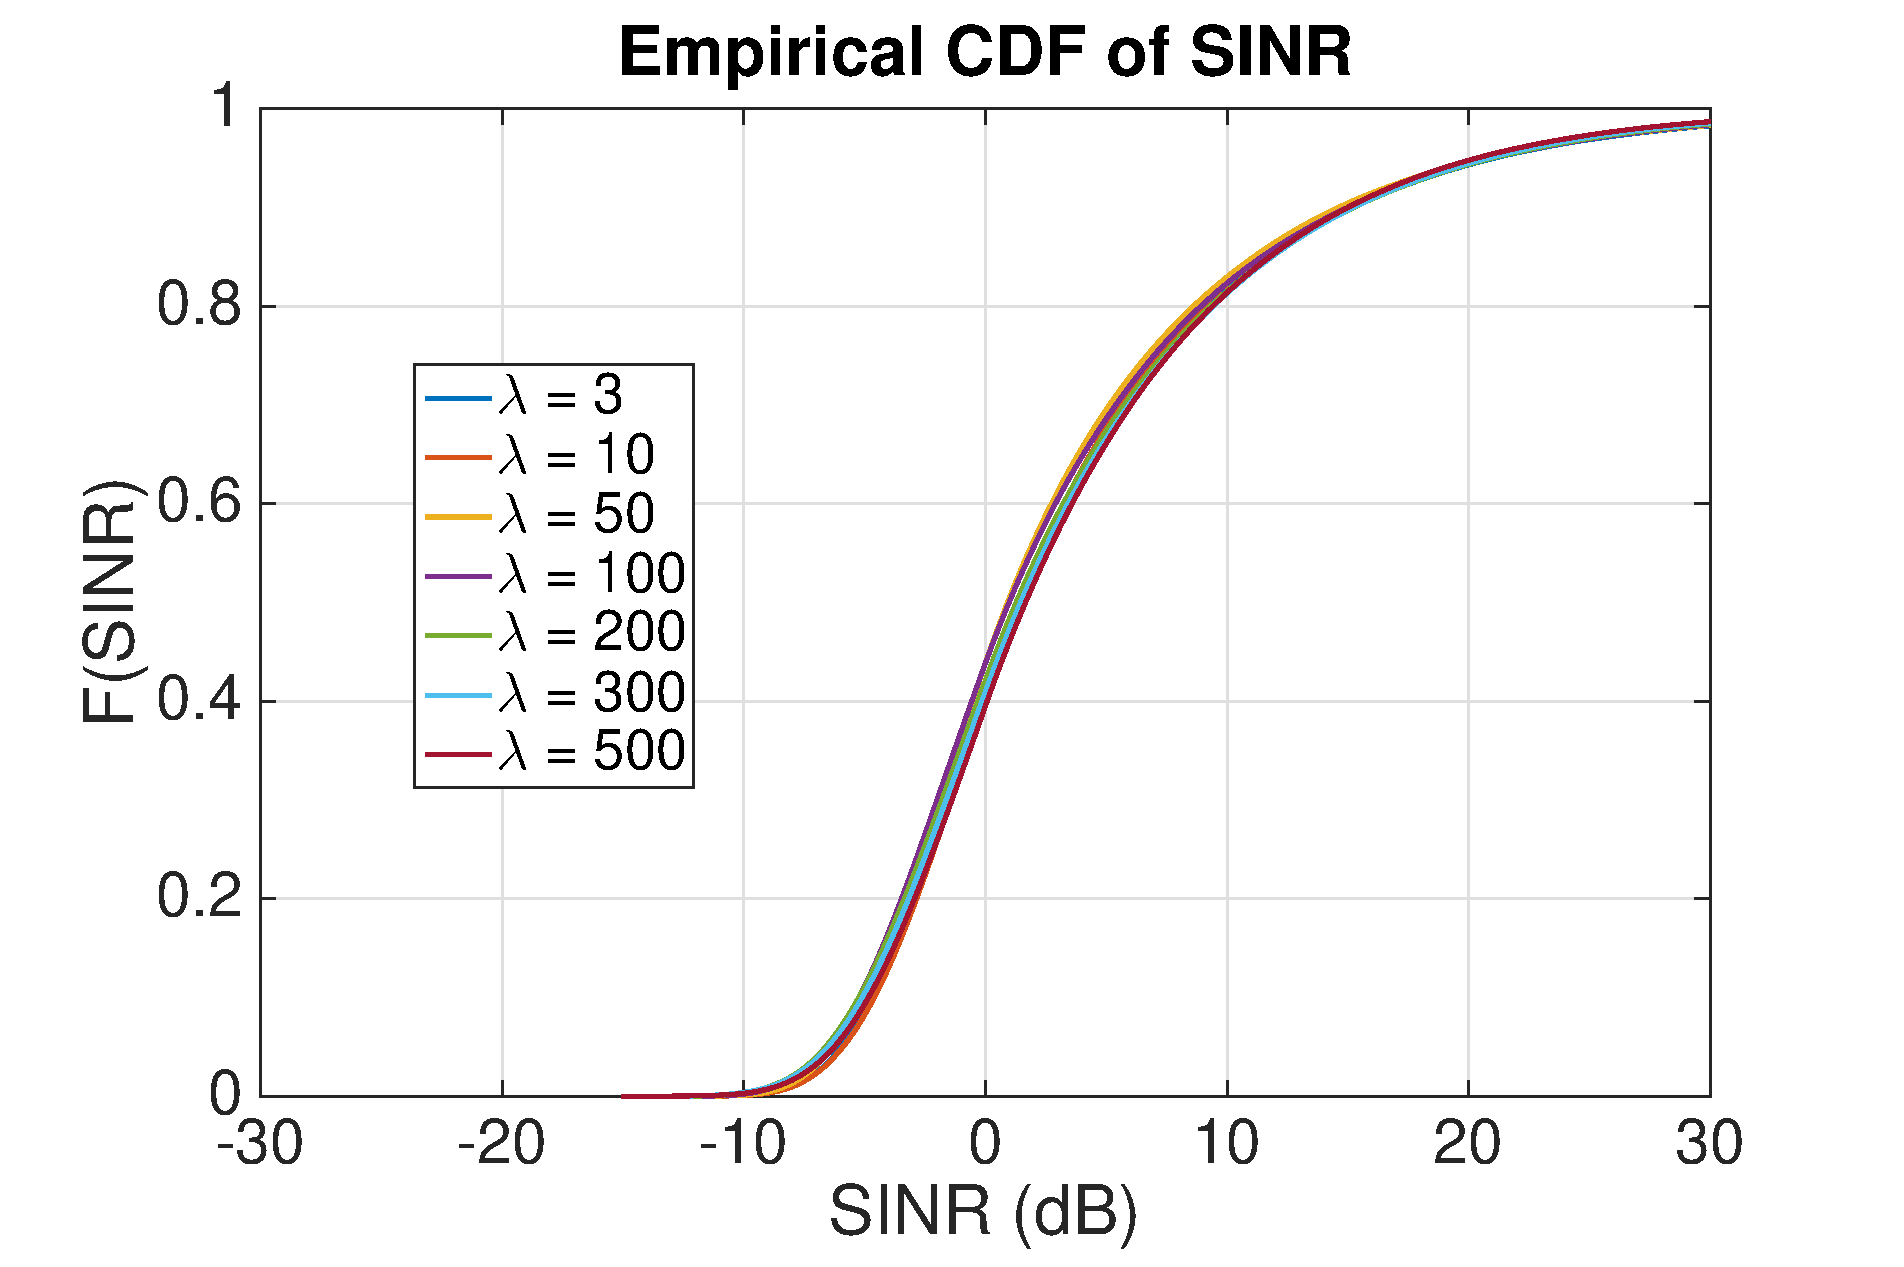
\includegraphics[width=10cm]{MaxMax1000OutageProbCDFDeCorr200.eps}
 \caption{CDF of SINR of MU when connecting to the strongest BS. De-Correlation Distance: 200m}
 \label{4:Mode32}
 \end{figure}

 \par For Random model, SINR distribution and outage probability of different BS densities are investigated for both Nearest BS mode and Strongest BS mode. Simulations are run for independent shadow fading and correlated shadow fading. CDF curves of SINR are generated and outage probability given SINR threshold being $-5dB$ are presented for increasing BS densities. Figure \ref{4:Mode1}, \ref{4:Mode2} and \ref{4:Mode3} shows the SINR of MU when connecting to the nearest BS. From Figure \ref{4:Mode1} and \ref{4:Mode2} we can see that the CDF curves are overlapping each other, which means increasing BS density does not change the CDF of SINR. From this we can conclude that when the shadow fading is independent or the de-correlation distance of the correlated shadow fading is small, increasing BS will not improve the system performance in terms of reducing outage probability. Figure \ref{4:Mode3}  illustrates that when increasing BS density, CDF of SINR improves (curve moves toward the bottom-right corner). This indicates that when de-correlation distance is large, increasing BS density will result in better system performance by reducing outage probability. Figure \ref{fig: outprob1} shows the outage probability of different correlated shadow fading models and different BS densities when SINR threshold is set to $-5dB$. Blue and green bars suggest that increasing BS density will not decrease outage probability when shadow fading is independent or correlated with $20m$ de-correlation distance. Yellow bars suggest that when the de-correlation distance is $200m$, increasing BS density will reduce outage probability. For example, when BS density is $3$, the outage probability is around $38\%$. Increasing BS density to $500$, the outage probability decreases to $18\%$. All above simulation results suggest that when de-correlation distance is relatively large and the MU is connecting to the nearest BS, increasing BS density will reduce outage probability and improve system performance.



 \begin{figure}
 \centering
 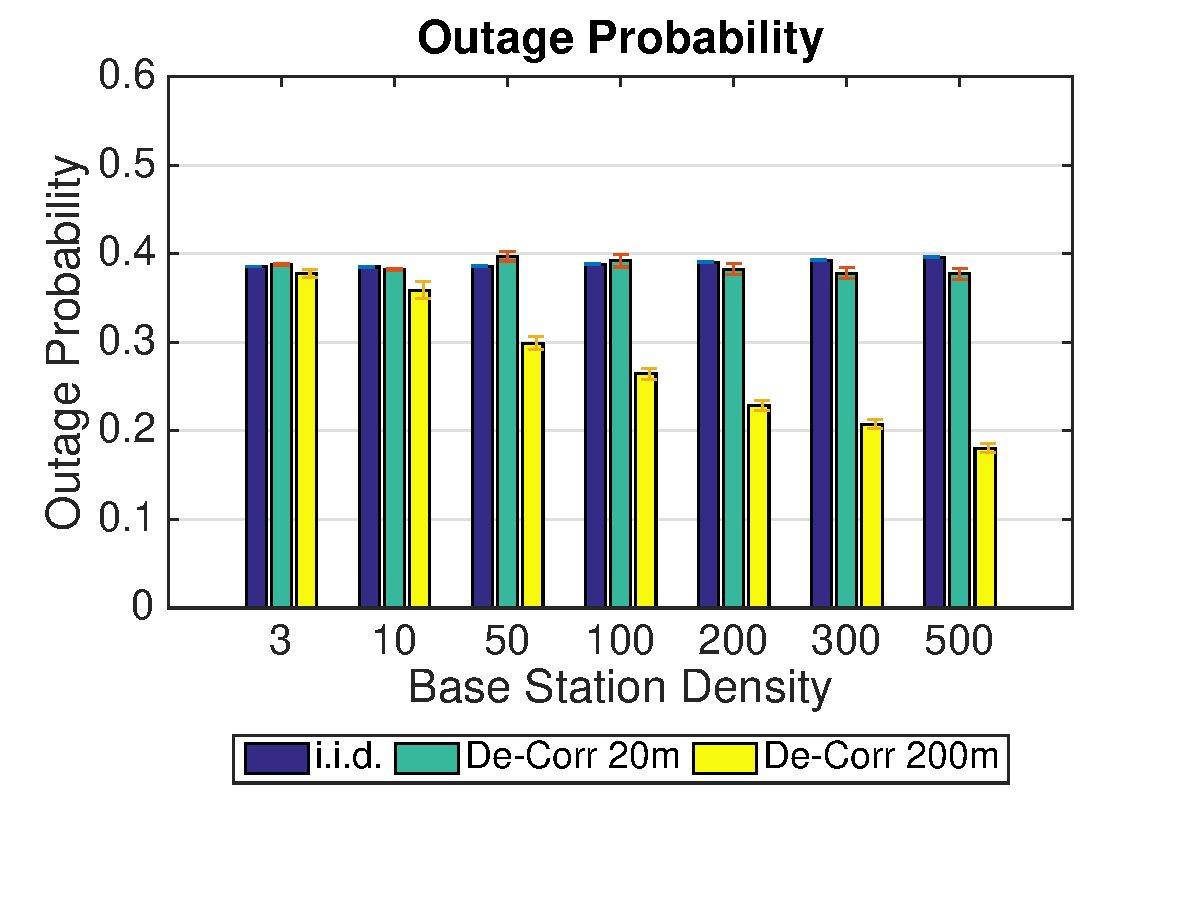
\includegraphics[width=10cm]{NBMax1000OutageProbThresh-5iid.eps}
 \caption{Outage probability given SINR threshold to be $-5dB$}
 \label{fig: outprob1}
 \end{figure}
 \begin{figure}
 \centering
 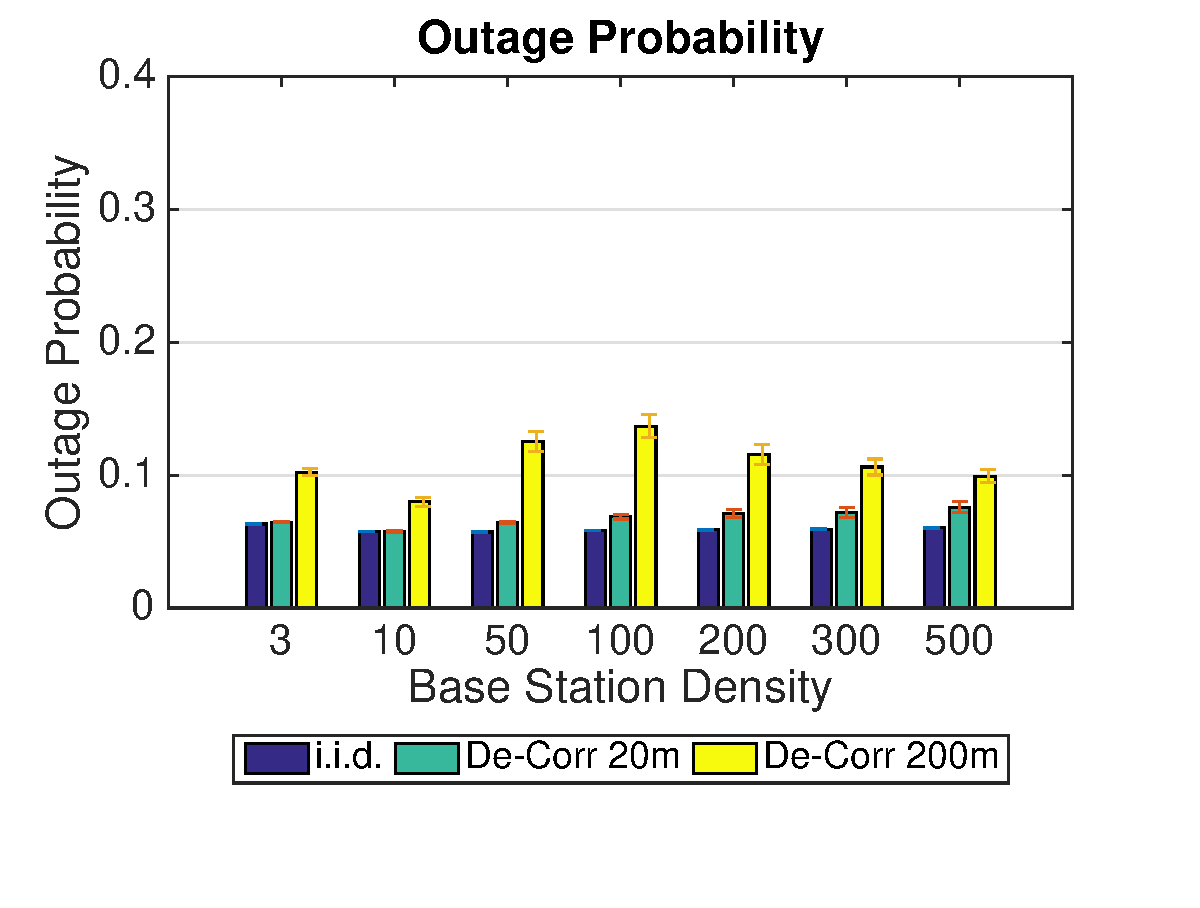
\includegraphics[width=10cm]{MaxMax1000OutageProbThresh-5iid.eps}
 \caption{Outage probability given SINR threshold to be $-5dB$}
 \label{fig: outprobs2}
 \end{figure}
 \begin{figure}
 \centering
 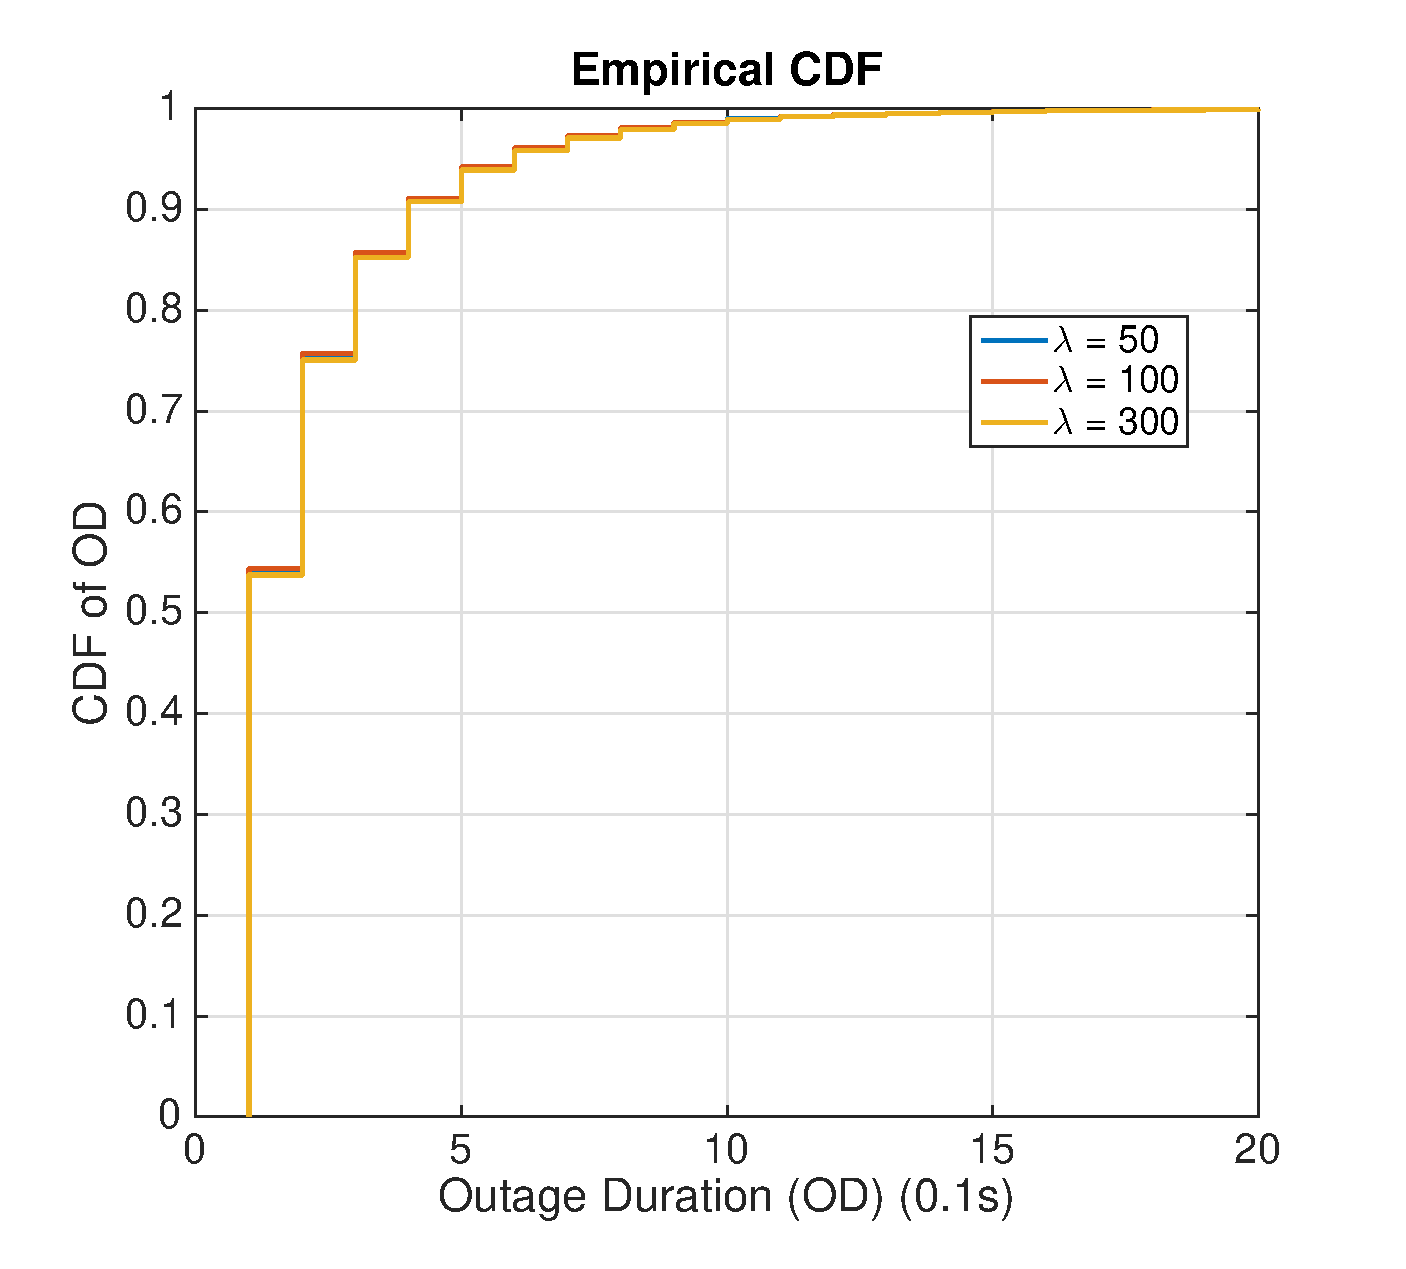
\includegraphics[width=10cm]{ODthresh-5iidNB.eps}
 \caption{CDF of Outage Duration of MU when connecting to the Nearest BS with i.i.d. shadowing}
 \label{iid1}
 \end{figure}
 \begin{figure}
 \centering
 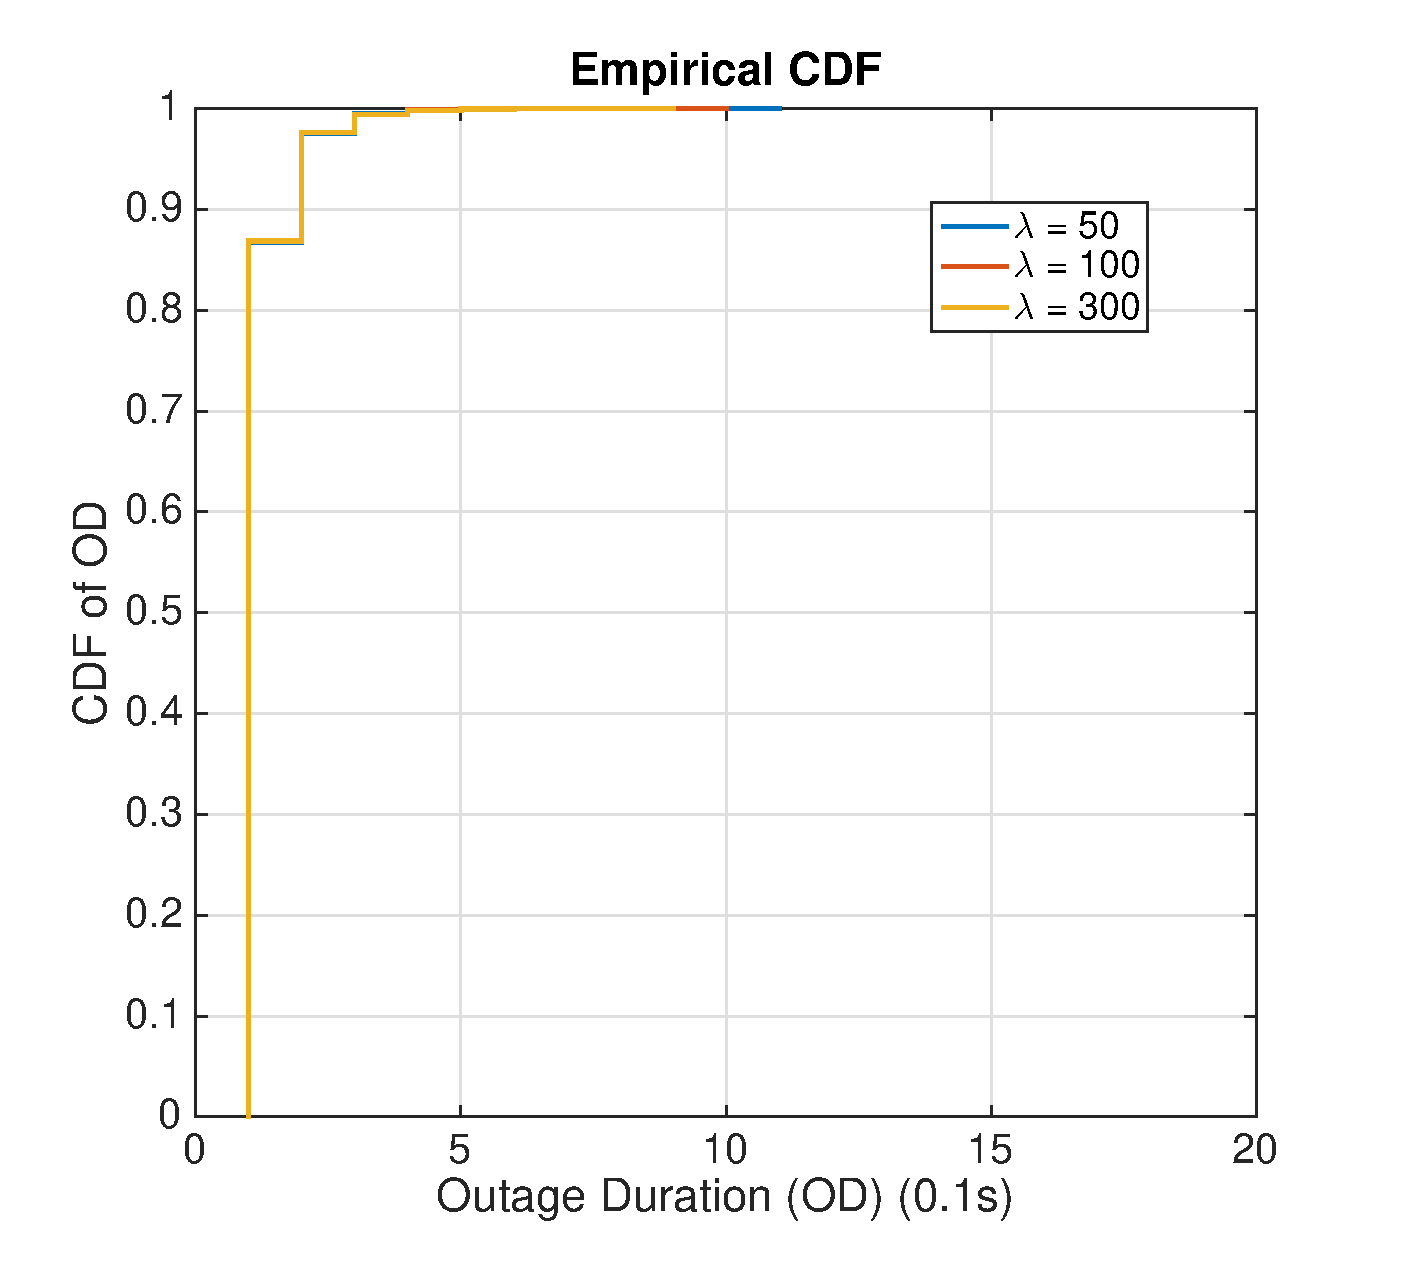
\includegraphics[width=10cm]{ODthresh-5iidMax.eps}
 \caption{CDF of Outage Duration of MU when connecting to the Strongest BS with i.i.d. shadowing}
 \label{iid2}
 \end{figure}
 \begin{figure}
 \centering
 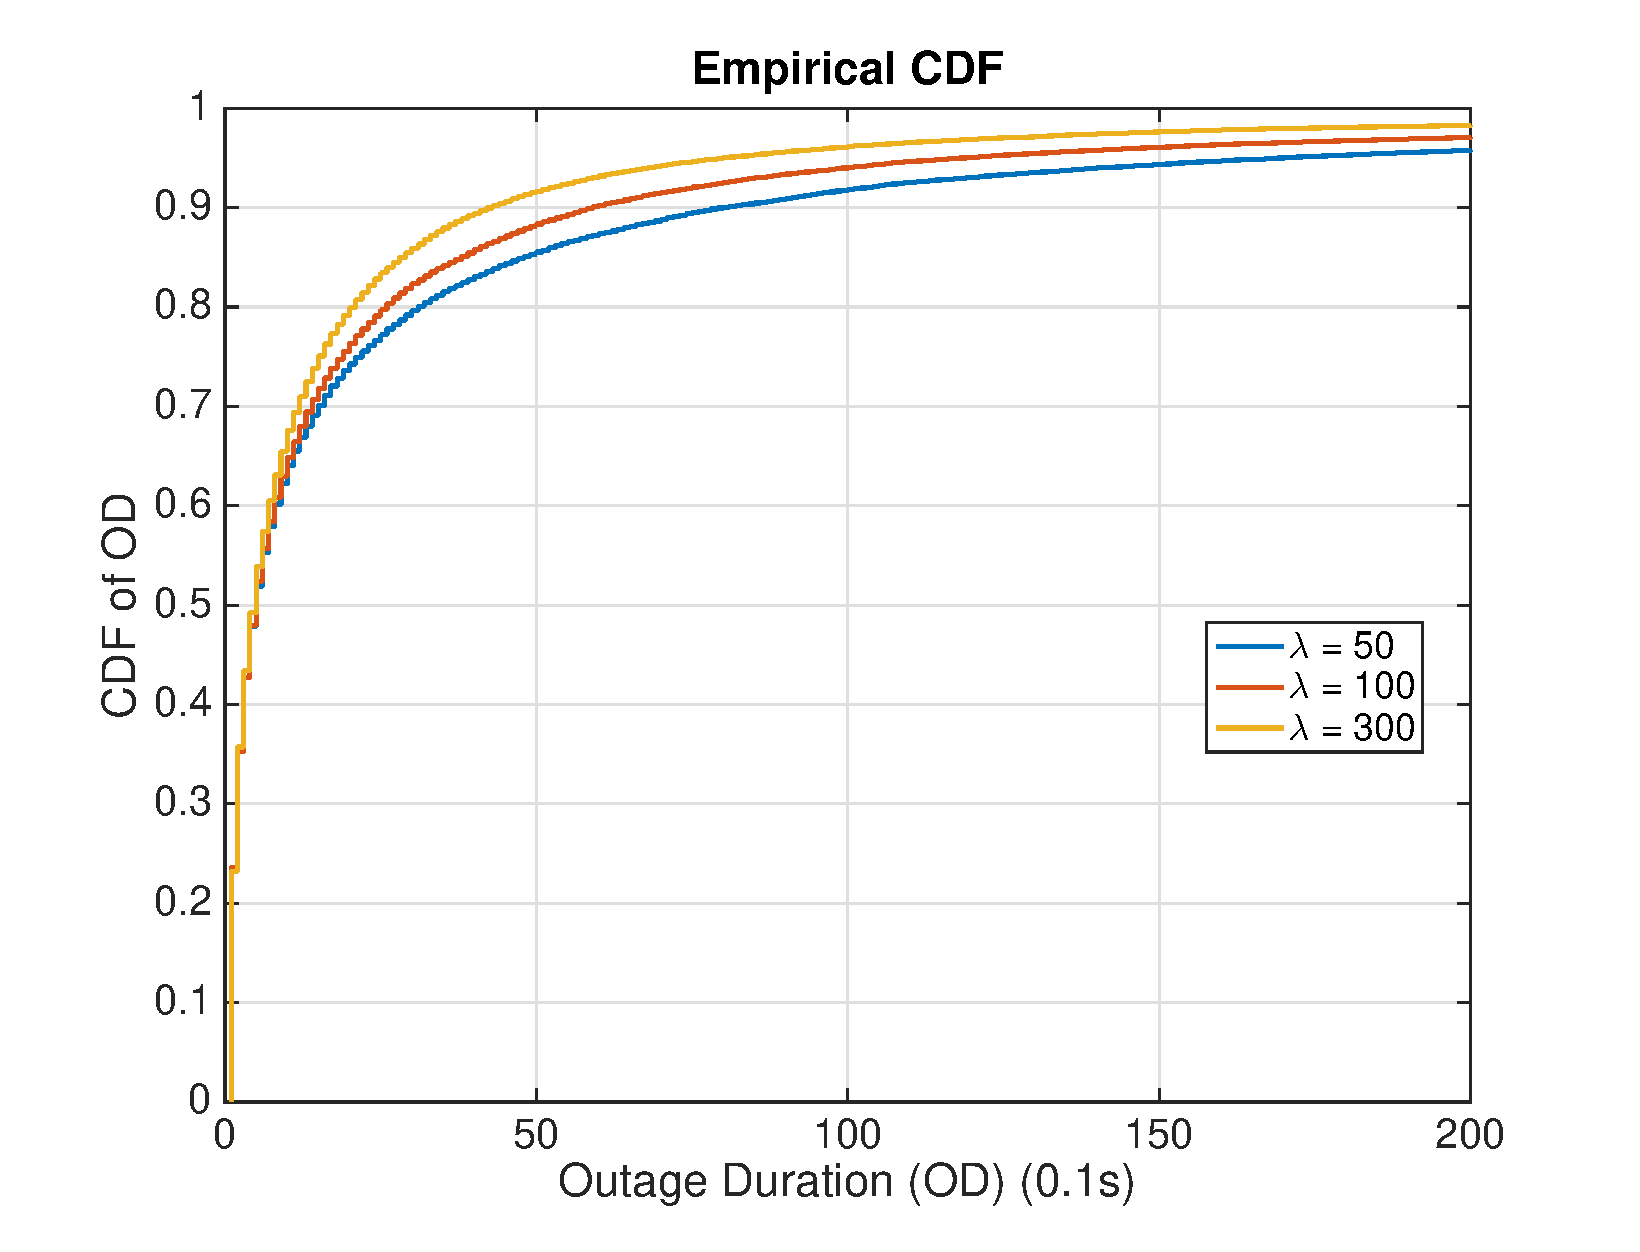
\includegraphics[width=10cm]{ODthresh-5DeCorr200NBMode2.eps}
 \caption{CDF of Outage Duration of MU when connecting to the Nearest BS with correlated shadowing (De-Correlation distance: 200m)}
 \label{corr1}
 \end{figure}
 \begin{figure}
 \centering
 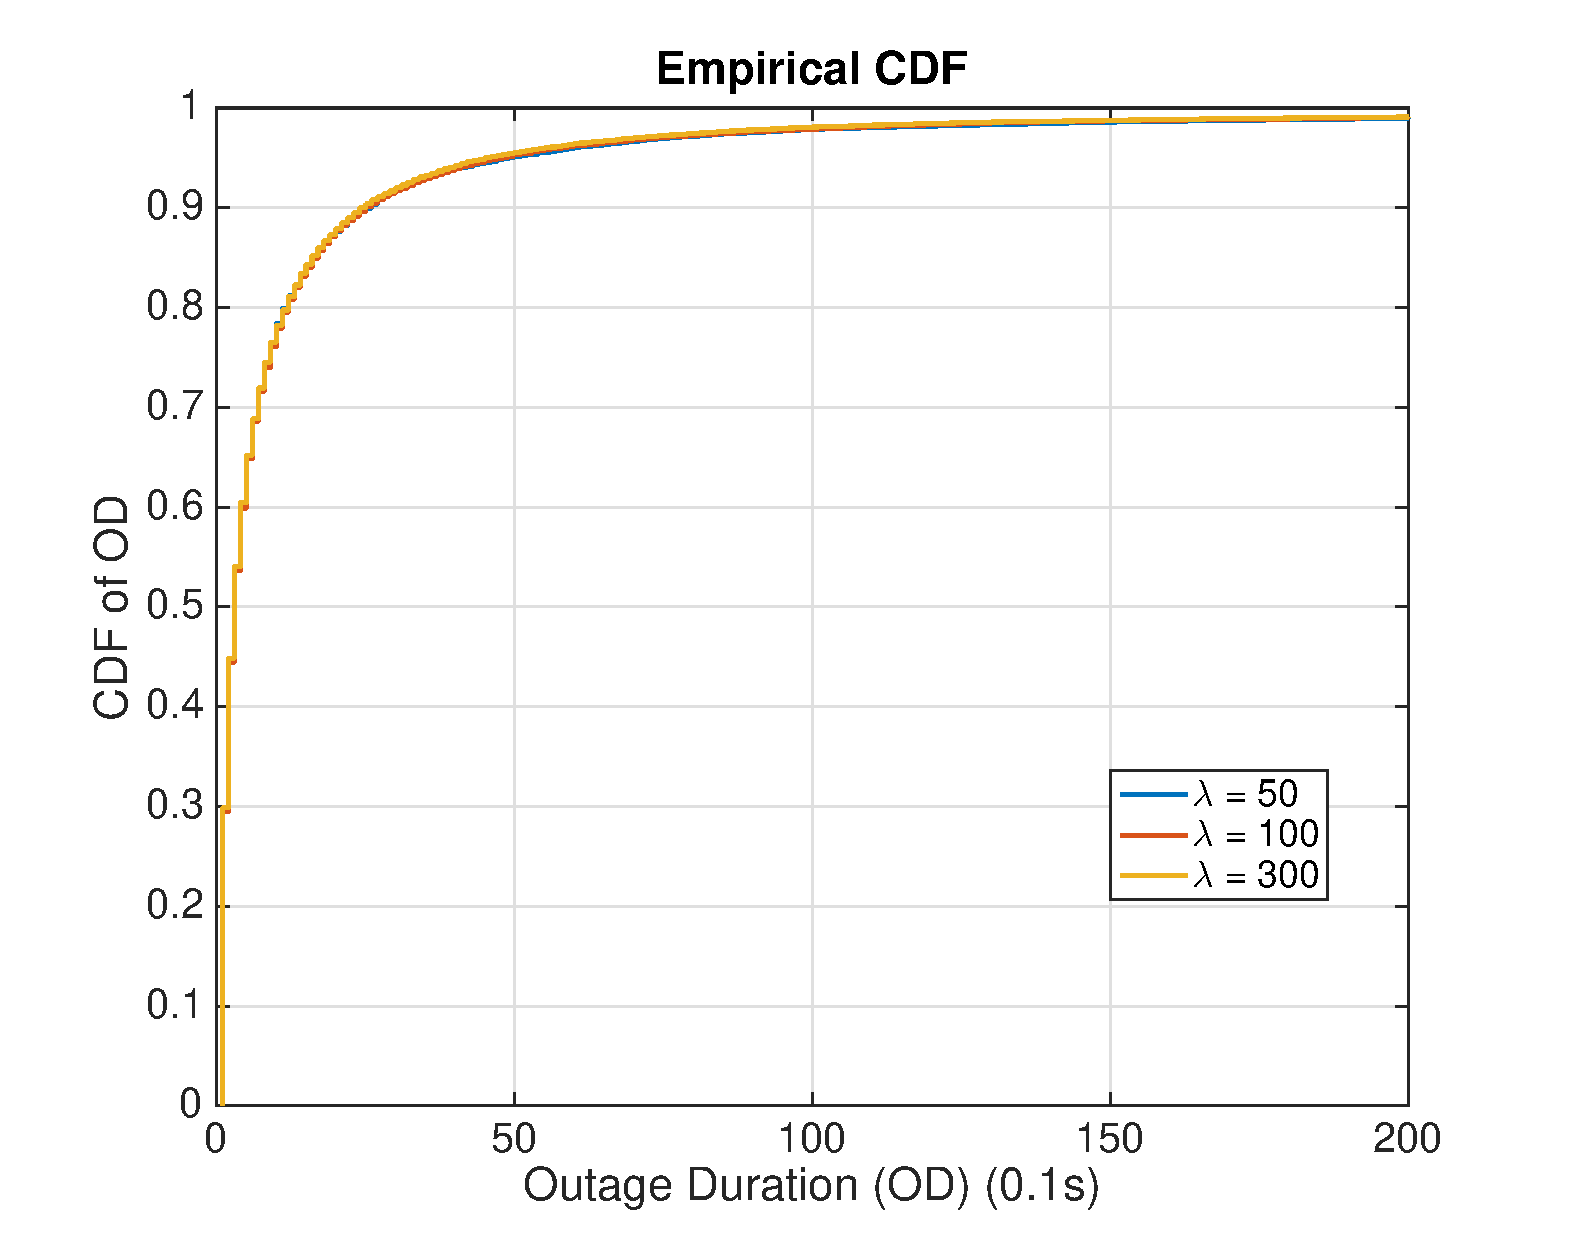
\includegraphics[width=10cm]{ODthresh-5DeCorr200MaxMode2.eps}
 \caption{CDF of Outage Duration of MU when connecting to the Strongest BS with correlated shadowing (De-Correlation distance: 200m)}
 \label{corr2}
 \end{figure}
 \par Next we move forward to investigate the system performance when the MU chooses to connect to the BS which provides the highest SINR. Same simulations as the nearest BS scenario are executed to explore this scenario. Figure \ref{4:Mode12}, \ref{4:Mode22} and \ref{4:Mode32} present the SINR of MU when connecting to the strongest BS. From Figure \ref{4:Mode12}, \ref{4:Mode22} and \ref{4:Mode32} we can see that CDF curves of SINR almost overlap each other when increasing BS densities, which means increasing BS density will not change CDF of SINR significantly. Figure \ref{fig: outprobs2} shows outage probability result which is consistent with our conclusion. For each shadow fading model, the difference between highest outage probability and lowest outage probability is less than $5\%$. Comparing three different shadow fading models, we can conclude that when the MU is connecting to the strongest BS, long de-correlation distance will harm the system performance in terms of outage probability (yellow bars are higher than green or blue bars). 
 \par Comparing Figure \ref{fig: outprob1} and Figure \ref{fig: outprobs2}, we find that with same BS density, the outage probabilities are lower for every shadow fading model if MU is connecting to the strongest BS. For example, with independent shadow fading and BS density to be $50$, the outage probability of Nearest BS mode is $38\%$ while that of Strongest BS mode is $6\%$. For correlated shadow fading with de-correlation distance being $200m$ and the BS density being $50$, we find that the outage probability of Nearest BS mode is around $30\%$. This is higher than that of the Strongest BS mode, which is $14\%$. Therefore,we conclude that connecting to the BS which provides highest SINR will improve the system performance with regard to the same network setup. 








 \par In the end, we investigate the system performance form the prospect of outage duration. We use Random Waypoint mobility model to model the user mobility. The parameters of the Random WayPoint model is given in Table \ref{RWP}. The MU speed is assumed to be between $1m/s$ (pedestrian speed) and $20m/s$ (car speed). The MU pause interval is assumed to be uniformly distributed between $0s$ to $60s$. The simulation time is set to be $0.1s$, which means for every $0.1s$ we check the MU's SINR to determine if it is in the outage area or not. Simulation results are shown in Figure \ref{iid1}, \ref{corr1}, \ref{iid2} and \ref{corr2}. Comparing Figure \ref{iid1} and Figure \ref{corr1}, Figure \ref{iid2} and Figure \ref{corr2}, we can see that when the channel is experiencing independent shadow fading, the outage duration is usually less than $2s$. However,  when the channel is under correlated shadow fading with de-correlation distance equal to $200m$, the outage duration can be longer than $20s$. Therefore, we draw the conclusion that correlated shadow fading leads to long-lasting outage durations and harm the system performance. Comparing Figure \ref{iid1} and Figure \ref{iid2}, we find that connecting to strongest BS will reduce the outage duration. For example, the percentage of outage durations with length less than $0.5s$ is $94\%$ for Nearest BS strategy, while that  of Strongest BS strategy is $100\%$.  Figure \ref{corr1} and Figure \ref{corr2} confirms this conclusion in addition. For example, the percentage of outage durations less than $5s$ in Figure \ref{corr1} is $85\%$ with BS density being $50$. However, that percentage in Figure \ref{corr2} is increased to $95\%$. Furthermore, Figure \ref{corr1} indicates that increasing BS density will reduce the percentage of long-lasting outage durations if MU is connecting to the nearest BS. For example, in Figure \ref{corr1}, when the BS density increase from $50$ to $300$, the probability of outage duration longer than $5s$ is reduced from $15\%$ to $8\%$. In contrast, for independent shadow fading and correlated shadow fading with MU connecting to strongest BS, increase BS density will not change the distribution of outage durations, which is confirmed by Figure \ref{iid1}, Figure \ref{iid2} and Figure \ref{corr2}. All CDF curves of outage durations are the same with different BS densities. 
 \begin{table}
 \centering
 \caption{\label{RWP}Random Waypoint Mobility Model Parameters}

 \begin{tabular}{|c|c|}

 \hline
 Speed Interval & $1 - 20m/s$\\
 \hline
 Pause Interval & $0 - 60s$\\
 \hline
 Simulation Time & $0.1s$\\
 \hline
 \end{tabular}

 \end{table}

 \section{Chapter Summary}
 \label{4:Conclusion}
 Shadow fading is large-scale fading which can cause significant received power loss for a wide area. In general, shadow fading is considered to be independent log-normal to simplify the analysis. However, this is not the real case. In reality, shadow fading at two different positions are correlated to each other. Correlated shadow fading will result in correlated outage events and long-lasting outage durations. To investigate a multi-cell system performance given correlated shadow fading, simulations are run to study the outage probability and outage duration distribution. First of all, the probability of two different BS layout: Grid model and Random model are investigated. We find that Grid Layout performs better than Random Layout. Secondly, outage probability given different BS densities and two different connecting strategies: Nearest BS mode and Strongest BS mode, are simulated. We conclude that connecting to strongest BS will reduce the outage probability comparing with nearest BS from simulation results. Increasing BS density will not reduce outage probability when MU is connecting to the strongest BS. However, when MU is connecting to the nearest BS and the de-correlation distance of correlated shadow fading is large enough, increasing BS density will reduce the outage probability.  At last, we investigate the system performance in terms of outage duration. Simulation results show that correlated shadow fading will result in long-lasting outage durations. Increasing BS density will reduce the percentage of long-lasting outage durations if the MU choose to connect to the nearest BS. Therefore, we suggest dense BS layout might be a proper strategy for next generation mmWave communication networks with correlated shadow fading.
 

